% =============================================================================
% NexOS - Kapsamli Teknik Dokumantasyon
% =============================================================================

\documentclass[12pt,a4paper]{report}

% --- PAKETLER ---
\usepackage[utf8]{inputenc}
\usepackage[T1]{fontenc}
\usepackage{geometry}
\usepackage{graphicx}
\usepackage{listings}
\usepackage{xcolor}
\usepackage{hyperref}
\usepackage{fancyhdr}
\usepackage{tikz}
\usepackage{float}

\geometry{margin=2.5cm}

% --- TURKCE CEVIRI ---
\renewcommand{\contentsname}{Icindekiler}
\renewcommand{\chaptername}{Bolum}
\renewcommand{\figurename}{Sekil}
\renewcommand{\tablename}{Tablo}
\renewcommand{\lstlistingname}{Kod}

% --- RENK TANIMLARI ---
\definecolor{codegreen}{rgb}{0,0.6,0}
\definecolor{codegray}{rgb}{0.5,0.5,0.5}
\definecolor{codepurple}{rgb}{0.58,0,0.82}
\definecolor{backcolour}{rgb}{0.95,0.95,0.92}
\definecolor{darkblue}{rgb}{0.0,0.0,0.6}

% --- KOD STILI ---
\lstdefinestyle{cstyle}{
    backgroundcolor=\color{backcolour},
    commentstyle=\color{codegreen},
    keywordstyle=\color{darkblue}\bfseries,
    numberstyle=\tiny\color{codegray},
    stringstyle=\color{codepurple},
    basicstyle=\ttfamily\footnotesize,
    breakatwhitespace=false,
    breaklines=true,
    captionpos=b,
    keepspaces=true,
    numbers=left,
    numbersep=5pt,
    showspaces=false,
    showstringspaces=false,
    showtabs=false,
    tabsize=2,
    language=C,
    frame=single,
    rulecolor=\color{black}
}

\lstdefinestyle{bashstyle}{
    backgroundcolor=\color{backcolour},
    commentstyle=\color{codegreen},
    keywordstyle=\color{darkblue}\bfseries,
    basicstyle=\ttfamily\footnotesize,
    breaklines=true,
    frame=single,
    language=bash
}

\lstset{style=cstyle}

% --- SAYFA BASLIGI ---
\pagestyle{fancy}
\fancyhf{}
\fancyhead[L]{NexOS Dokumantasyonu}
\fancyhead[R]{\thepage}
\fancyfoot[C]{Teknik Dokumantasyon}

% --- BELGE BASLANGICI ---
\begin{document}

% =============================================================================
% KAPAK SAYFASI
% =============================================================================
\begin{titlepage}
    \centering
    \vspace*{2cm}
    
    
\includegraphics[width=1.0\textwidth]{nexos_cover.png}\\[1.5cm]
    
    {\large Kapsamlı Teknik Dokümantasyon}\\[2cm]
    
    \vspace{3cm}
    
    {\large\textbf{Hazirlayanlar:}}\\[0.3cm]
    {\normalsize MASIHULLAH OMAR (170422921)}\\[0.2cm]
    {\normalsize ALİ RIZA MISTIK (170423851)}\\[1cm]
    

    
    \vfill
    
    {\large Tarih: 30 Aral{\i}k 2025}
    
\end{titlepage}

% =============================================================================
% ICINDEKILER
% =============================================================================
\tableofcontents
\newpage

% =============================================================================
% BOLUM 1: GIRIS
% =============================================================================
\chapter{Giriş}

\section{NexOS Nedir?}

\textbf{NexOS}, modern işletim sistemi kavramlarını gösteren eğitim amaçlı bir sistemdir. Kullanıcılara:

\begin{itemize}
    \item Süreç yönetimi ve izolasyon
    \item Bellek tahsisi ve koruma
    \item CPU zamanlama algoritmaları
    \item Dosya sistemi işlemleri
    \item Web sunucu yönetimi ve log analizi
    \item Yapay zeka destekli komut asistanı
\end{itemize}

konularında pratik deneyim sağlar.

\section{Yapay Zeka Entegrasyonu}

NexOS, kullanıcılara komut önerilerinde bulunmak için entegre bir yapay zeka asistanı içerir. Bu asistan:

\begin{itemize}
    \item \textbf{Ollama} acik kaynak AI calisma zamanini kullanir
    \item \textbf{Qwen 1.5B} modelini temel alir (1.5 milyar parametre)
    \item Ozel veri seti uzerinde \textbf{fine-tune} edilmistir
    \item BusyBox komutlarini onerme konusunda uzmanlasmistir
    \item Tehlikeli komutlari filtreleyerek guvenlik saglar
\end{itemize}

Fine-tuning sureci, modelin NexOS ortamina ozgu komutlari daha dogru onermesini saglar. Model, GGUF formatinda paketlenerek ISO icine dahil edilir ve internet baglantisi gerektirmeden yerel olarak calisir.

\section{Temel Kavramlar}

\subsection{Süreç (Process)}

Bir \textbf{süreç}, çalıştırılan bir programdır. Her süreç:
\begin{itemize}
    \item Benzersiz bir PID (Process ID) numarasına sahiptir
    \item Kendi izole bellek alanında çalışır
    \item Farklı durumlarda (NEW, READY, RUNNING, BLOCKED, TERMINATED) bulunabilir
\end{itemize}

\subsection{Bellek İzolasyonu}

Her süreç kendi özel bellek alanına sahiptir. Bir süreç, başka bir sürecin belleğine erişemez. Bu güvenlik için kritik öneme sahiptir.

\subsection{Zamanlayıcı (Scheduler)}

CPU aynı anda sadece bir süreç çalıştırır. \textbf{Zamanlayıcı}, hangi sürecin ne zaman çalışacağına karar verir. NexOS, \textbf{Round-Robin} algoritmasını kullanır.

\section{Sistem Gereksinimleri}

NexOS çalıştırmak için:
\begin{itemize}
    \item GCC derleyici (statik derleme destekli)
    \item Make (derleme otomasyonu)
    \item QEMU veya VirtualBox (ISO test için)
    \item xorriso (ISO oluşturma)
    \item wget ve curl (BusyBox/Ollama indirme)
    \item 2GB RAM ve 5GB disk alanı (önerilen)
\end{itemize}

% =============================================================================
% BOLUM 1.5: GELISTIRME ORTAMI
% =============================================================================
\chapter{Geliştirme Ortamı Kurulumu}

\section{Bağımlılıkların Kurulumu}

\subsection{Ubuntu/Debian}

\begin{lstlisting}[style=bashstyle,caption={Gerekli Paketlerin Kurulumu}]
# Temel derleme araclari
sudo apt update
sudo apt install -y build-essential gcc make

# Statik derleme icin gerekli
sudo apt install -y libc6-dev libgcc-s1

# ISO olusturma araclari
sudo apt install -y xorriso isolinux syslinux-common

# Sanal makine (QEMU)
sudo apt install -y qemu-system-x86

# Indirme araclari
sudo apt install -y wget curl
\end{lstlisting}

\subsection{Fedora/RHEL}

\begin{lstlisting}[style=bashstyle,caption={Fedora Kurulumu}]
sudo dnf install -y gcc make glibc-static
sudo dnf install -y xorriso syslinux
sudo dnf install -y qemu-system-x86
\end{lstlisting}

\subsection{macOS (Sadece Derleme)}

\begin{lstlisting}[style=bashstyle,caption={macOS Kurulumu}]
# Homebrew ile
brew install gcc make qemu

# NOT: macOS'ta statik derleme ve ISO
# olusturma icin Linux VM oneriliyor
\end{lstlisting}

\section{Proje Dizin Yapısı}

NexOS projesi aşağıdaki dizin yapısına sahiptir:

\begin{lstlisting}[style=bashstyle,caption={Proje Yapisi}]
nexos/
|
+-- src/                    # C kaynak kodlari
|   +-- globals.h           # Ortak tanimlamalar
|   +-- main.c              # Ana giris noktasi
|   +-- process.c           # Surec yonetimi
|   +-- memory.c            # Bellek yonetimi
|   +-- scheduler.c         # CPU zamanlayici
|   +-- ipc.c               # Surecler arasi iletisim
|   +-- fs.c                # Dosya sistemi
|   +-- shell.c             # Komut kabugu
|   +-- tui.c               # Terminal arayuzu
|   +-- hardware.c          # Donanim bilgileri
|   +-- utils.c             # Yardimci fonksiyonlar
|   +-- ai.c                # AI entegrasyonu
|
+-- scripts/                # Shell scriptleri
|   +-- webserver.sh        # Web sunucu
|   +-- log_analyzer.sh     # Log analizi
|   +-- analyze_traffic.sh  # Trafik analizi
|
+-- distro/                 # ISO olusturma
|   +-- build_iso.sh        # Ana build scripti
|   +-- init                # Boot scripti
|
+-- Makefile                # Derleme kurallari
+-- README.md               # Proje aciklamasi
\end{lstlisting}

\section{Projeyi Sıfırdan Oluşturma}

\subsection{Adım 1: Proje Dizinini Oluştur}

\begin{lstlisting}[style=bashstyle]
mkdir -p nexos/src nexos/scripts nexos/distro
cd nexos
\end{lstlisting}

\subsection{Adım 2: Makefile Oluştur}

\begin{lstlisting}[style=bashstyle,caption={Makefile}]
# Derleyici ayarlari
CC = gcc
CFLAGS = -Wall -Wextra -static -O2

# Dizinler
SRCDIR = src
BUILDDIR = build

# Kaynak dosyalari
SOURCES = main.c process.c memory.c scheduler.c \
          ipc.c fs.c shell.c tui.c hardware.c \
          utils.c ai.c
OBJECTS = $(SOURCES:.c=.o)

# Ana hedef
all: nexos

nexos: $(OBJECTS)
	$(CC) $(CFLAGS) -o $@ $(addprefix $(SRCDIR)/,$^)

# C dosyalarini derle
%.o: $(SRCDIR)/%.c $(SRCDIR)/globals.h
	$(CC) $(CFLAGS) -c $< -o $(SRCDIR)/$@

# Temizlik
clean:
	rm -f $(SRCDIR)/*.o nexos

# ISO olustur
iso: nexos
	cd distro && ./build_iso.sh

.PHONY: all clean iso
\end{lstlisting}

\section{globals.h - Merkezi Tanımlamalar}

Tüm modüller \texttt{globals.h} dosyasını include eder. Bu dosya projenin ``anayasası'' gibidir.

\subsection{Header Guard ve Kütüphane Bildirimleri}

\begin{lstlisting}[caption={globals.h - Baslangic}]
#ifndef GLOBALS_H
#define GLOBALS_H

// Standart C kutuphaneleri
#include <stdio.h>      // printf, scanf, FILE
#include <stdlib.h>     // malloc, free, exit
#include <string.h>     // strcpy, strcmp, memset
#include <unistd.h>     // read, write, access
#include <stdbool.h>    // true, false, bool
#include <sys/sysinfo.h>// Sistem bilgileri
#include <sys/statvfs.h>// Disk bilgileri
#include <termios.h>    // Terminal kontrolu
#include <time.h>       // Zaman fonksiyonlari
\end{lstlisting}

\subsection{Sabit Tanımlamalar}

\begin{lstlisting}[caption={globals.h - Sabitler}]
// Versiyon bilgisi
#define NEXOS_VERSION "1.2.0"

// Terminal renk kodlari (ANSI)
#define RENK_KIRMIZI "\033[1;31m"
#define RENK_YESIL   "\033[1;32m"
#define RENK_MAVI    "\033[1;34m"
#define RENK_SARI    "\033[1;33m"
#define RENK_CYAN    "\033[1;36m"
#define RENK_SIFIRLA "\033[0m"

// Dosya sistemi ayarlari
#define DISK_DOSYASI "sanal_disk.bin"
#define MAX_DOSYA 50
#define MAX_DOSYA_BOYUTU 1024

// Surec ve bellek ayarlari
#define MAX_PROCESS 10
#define PROCESS_MEMORY_SIZE 4096  // 4KB
#define TIME_QUANTUM 3            // Round-Robin
#define MAX_IPC_MESSAGES 10
#define MAX_IPC_MSG_SIZE 256
\end{lstlisting}

\subsection{Enum Tanımlamaları}

\begin{lstlisting}[caption={globals.h - Enumlar}]
// Surec durumlari
typedef enum {
    PROC_NEW,        // Yeni olusturuldu
    PROC_READY,      // Hazir
    PROC_RUNNING,    // Calisiyor
    PROC_BLOCKED,    // Bloklu
    PROC_TERMINATED  // Sonlandi
} ProcessState;
\end{lstlisting}

\subsection{Veri Yapıları}

\begin{lstlisting}[caption={globals.h - Struct Tanimlamalari}]
// IPC Mesaj yapisi
typedef struct {
    int sender_pid;
    int receiver_pid;
    char content[MAX_IPC_MSG_SIZE];
    bool read;
} IPCMessage;

// Surec kontrol blogu (PCB)
typedef struct {
    int pid;
    char name[32];
    ProcessState state;
    int priority;
    int time_slice;
    
    // Izole bellek
    int memory_base;
    int memory_limit;
    char memory_space[PROCESS_MEMORY_SIZE];
    int memory_used;
    
    // IPC
    IPCMessage mailbox[MAX_IPC_MESSAGES];
    int mailbox_count;
    
    bool active;
} SimProcess;

// Dosya sistemi blogu
typedef struct {
    char ad[32];
    int boyut;
    char icerik[MAX_DOSYA_BOYUTU];
    bool dolu;
} DosyaBlogu;
\end{lstlisting}

\subsection{Global Değişkenler ve Fonksiyon Prototipleri}

\begin{lstlisting}[caption={globals.h - Extern ve Prototipler}]
// Global tablo (tum moduller erisebilir)
extern SimProcess process_table[MAX_PROCESS];
extern DosyaBlogu sanal_disk[MAX_DOSYA];
extern int pid_counter;

// === FONKSIYON PROTOTIPLERI ===

// process.c
SimProcess* process_create(char *name, int priority);
void process_terminate(int pid);
SimProcess* process_find(int pid);
void process_list();
void process_block(int pid);
void process_unblock(int pid);

// memory.c
void memory_init();
int mem_write(int pid, int offset, void *data, int size);
int mem_read(int pid, int offset, void *buffer, int size);
void mem_demo();

// scheduler.c
void scheduler_init();
void scheduler_tick();
void scheduler_demo();

// ipc.c
int ipc_send(int sender, int receiver, char *msg);
int ipc_receive(int pid, char *buffer);
void ipc_demo();

// fs.c
void sfs_yukle();
void sfs_kaydet();
void sfs_dosya_olustur(char *isim, char *icerik);
void sfs_liste();

// shell.c
void shell_run();

// tui.c
int show_login_screen();
void tui_menu();

// ai.c
void ai_sor(char *soru);
void ai_command_helper_run(char *soru);

#endif // GLOBALS_H
\end{lstlisting}

\section{main.c - Program Giriş Noktası}

\begin{lstlisting}[caption={main.c - Temel Yapi}]
#include "globals.h"
#include <signal.h>

// Global degiskenlerin tanimlari
SimProcess process_table[MAX_PROCESS];
DosyaBlogu sanal_disk[MAX_DOSYA];
int pid_counter = 1000;

// Sinyal handler (temiz cikis)
void handle_signal(int sig) {
    printf("\nNexOS kapatiliyor...\n");
    sfs_kaydet();  // Dosya sistemini kaydet
    exit(0);
}

int main() {
    // Sinyal yakala
    signal(SIGINT, handle_signal);
    signal(SIGTERM, handle_signal);
    
    // Sistemleri baslat
    sfs_yukle();    // Dosya sistemi
    memory_init();  // Bellek simulasyonu
    
    // Giris ekrani
    if (show_login_screen() != 0) {
        printf("Giris basarisiz!\n");
        return 1;
    }
    
    // Ana menu
    tui_menu();
    
    // Cikista kaydet
    sfs_kaydet();
    
    return 0;
}
\end{lstlisting}

\section{Derleme ve Test}

\begin{lstlisting}[style=bashstyle,caption={Proje Derleme}]
# Dizine git
cd nexos

# Derle
make

# Calistir (normal mod)
./nexos

# ISO olustur (Linux gerekli)
make iso

# QEMU ile test
qemu-system-x86_64 -cdrom distro/nexos.iso -m 2G
\end{lstlisting}

% =============================================================================
% BOLUM 2: SISTEM MIMARISI
% =============================================================================
\chapter{Sistem Mimarisi}

\section{Genel Bakış}

NexOS modüler bir yapıya sahiptir. Her modül belirli bir görev üstlenir:

\begin{figure}[h]
\centering
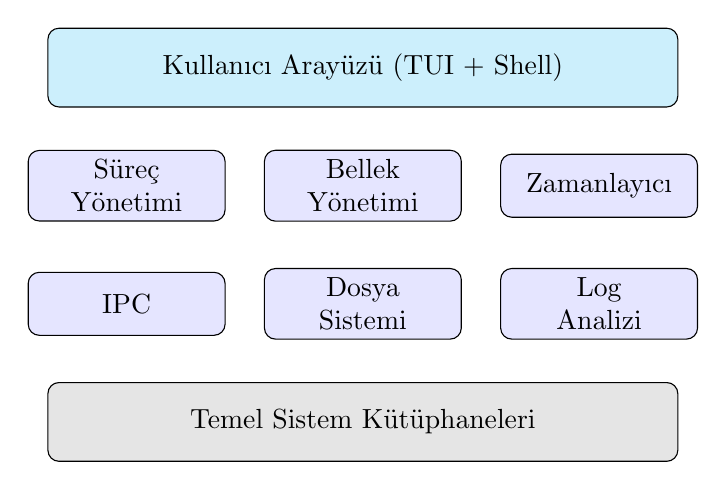
\begin{tikzpicture}[
    box/.style={rectangle, draw, rounded corners, minimum width=2.5cm, minimum height=0.8cm, align=center, fill=blue!10},
    bigbox/.style={rectangle, draw, rounded corners, minimum width=8cm, minimum height=1cm, align=center, fill=green!10}
]
    % User Interface Layer
    \node[bigbox, fill=cyan!20] at (0,4) {Kullanıcı Arayüzü (TUI + Shell)};
    
    % Core modules
    \node[box] at (-3,2.5) {Süreç\\Yönetimi};
    \node[box] at (0,2.5) {Bellek\\Yönetimi};
    \node[box] at (3,2.5) {Zamanlayıcı};
    
    \node[box] at (-3,1) {IPC};
    \node[box] at (0,1) {Dosya\\Sistemi};
    \node[box] at (3,1) {Log\\Analizi};
    
    % Base
    \node[bigbox, fill=gray!20] at (0,-0.5) {Temel Sistem Kütüphaneleri};
    
\end{tikzpicture}
\caption{NexOS Sistem Mimarisi}
\end{figure}

\section{Kaynak Dosyaları}

\begin{tabular}{|l|l|}
\hline
\textbf{Dosya} & \textbf{Görevi} \\
\hline
\texttt{main.c} & Program giriş noktası \\
\texttt{globals.h} & Global tanımlamalar \\
\texttt{process.c} & Süreç oluşturma ve yönetimi \\
\texttt{memory.c} & İzole bellek işlemleri \\
\texttt{scheduler.c} & Round-Robin zamanlayıcı \\
\texttt{ipc.c} & Süreçler arası mesajlaşma \\
\texttt{fs.c} & Sanal dosya sistemi \\
\texttt{shell.c} & Komut satırı arayüzü \\
\texttt{tui.c} & Terminal grafik arayüzü \\
\texttt{utils.c} & Yardımcı fonksiyonlar \\
\hline
\end{tabular}

\section{Derleme ve Çalıştırma}

\begin{lstlisting}[style=bashstyle,caption={Derleme Komutlari}]
# Binary derleme
make

# ISO olusturma
make iso

# QEMU ile calistirma
qemu-system-x86_64 -cdrom distro/nexos.iso -m 2G
\end{lstlisting}

\section{Katmanlı Mimari}

NexOS, katmanlı bir mimari yaklaşımı benimser. Üst katmanlar alt katmanların sunduğu servisleri kullanır:

\begin{figure}[h]
\centering
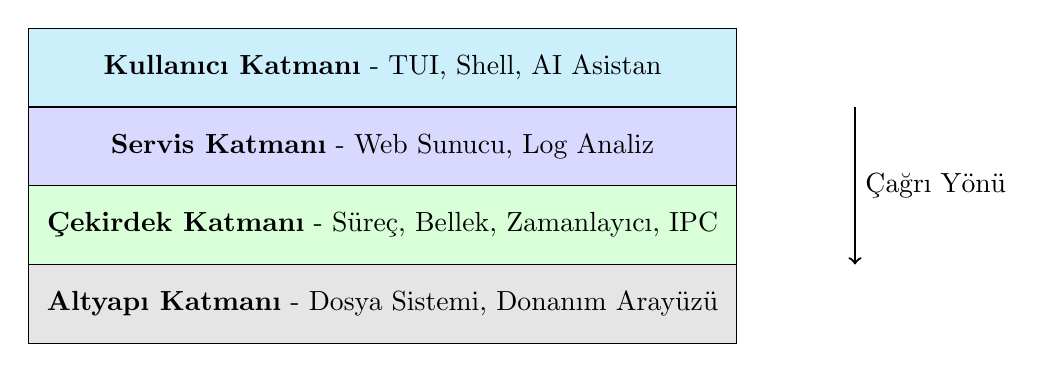
\begin{tikzpicture}[
    layer/.style={rectangle, draw, minimum width=9cm, minimum height=1cm, align=center}
]
    \node[layer, fill=cyan!20] at (0,3) {\textbf{Kullanıcı Katmanı} - TUI, Shell, AI Asistan};
    \node[layer, fill=blue!15] at (0,2) {\textbf{Servis Katmanı} - Web Sunucu, Log Analiz};
    \node[layer, fill=green!15] at (0,1) {\textbf{Çekirdek Katmanı} - Süreç, Bellek, Zamanlayıcı, IPC};
    \node[layer, fill=gray!20] at (0,0) {\textbf{Altyapı Katmanı} - Dosya Sistemi, Donanım Arayüzü};
    
    \draw[->, thick] (6,2.5) -- (6,0.5) node[midway, right] {Çağrı Yönü};
\end{tikzpicture}
\caption{NexOS Katmanlı Mimari}
\end{figure}

\section{Veri Akışı}

Sistem içerisindeki temel veri akışı şu şekilde gerçekleşir:

\begin{figure}[h]
\centering
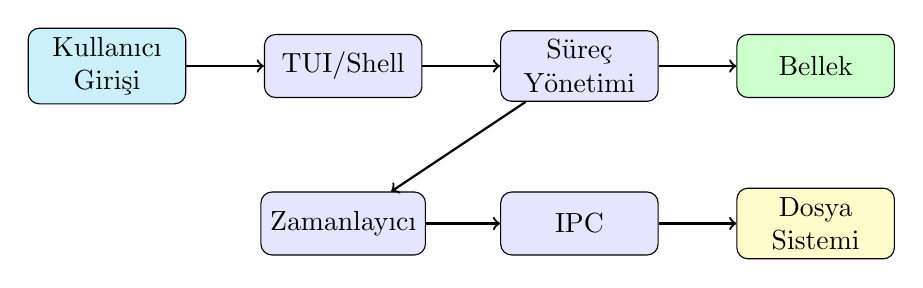
\begin{tikzpicture}[
    box/.style={rectangle, draw, rounded corners, minimum width=2cm, minimum height=0.8cm, align=center, fill=blue!10},
    arrow/.style={->, thick}
]
    % User Input
    \node[box, fill=cyan!20] (input) at (0,0) {Kullanıcı\\Girişi};
    \node[box] (tui) at (3,0) {TUI/Shell};
    \node[box] (process) at (6,0) {Süreç\\Yönetimi};
    \node[box, fill=green!20] (memory) at (9,0) {Bellek};
    
    \draw[arrow] (input) -- (tui);
    \draw[arrow] (tui) -- (process);
    \draw[arrow] (process) -- (memory);
    
    % Second row
    \node[box] (scheduler) at (3,-2) {Zamanlayıcı};
    \node[box] (ipc) at (6,-2) {IPC};
    \node[box, fill=yellow!20] (fs) at (9,-2) {Dosya\\Sistemi};
    
    \draw[arrow] (process) -- (scheduler);
    \draw[arrow] (scheduler) -- (ipc);
    \draw[arrow] (ipc) -- (fs);
    
\end{tikzpicture}
\caption{Sistem Veri Akisi}
\end{figure}

\section{Modül Etkileşim Matrisi}

Aşağıdaki tablo hangi modülün hangi modülü kullandığını gösterir:

\begin{center}
\begin{tabular}{|l|c|c|c|c|c|c|}
\hline
\textbf{Modül} & \textbf{process} & \textbf{memory} & \textbf{sched} & \textbf{ipc} & \textbf{fs} & \textbf{shell} \\
\hline
shell.c & X & X & X & X & X & - \\
tui.c & X & - & - & - & - & X \\
scheduler.c & X & - & - & - & - & - \\
ipc.c & X & - & - & - & - & - \\
ai.c & - & - & - & - & - & X \\
\hline
\end{tabular}
\end{center}

\section{Merkezi Header Dosyası}

Tum moduller \texttt{globals.h} dosyasini dahil eder. Bu dosya:

\begin{itemize}
    \item Paylaşılan veri yapılarını tanımlar (\texttt{SimProcess}, \texttt{DosyaBlogu})
    \item Sistem sabitlerini belirler (\texttt{MAX\_PROCESS}, \texttt{TIME\_QUANTUM})
    \item Fonksiyon prototiplerini bildirir (modüller arası çağrılar için)
    \item ANSI renk kodlarını tanımlar (terminal çıktısı için)
\end{itemize}

\begin{figure}[h]
\centering
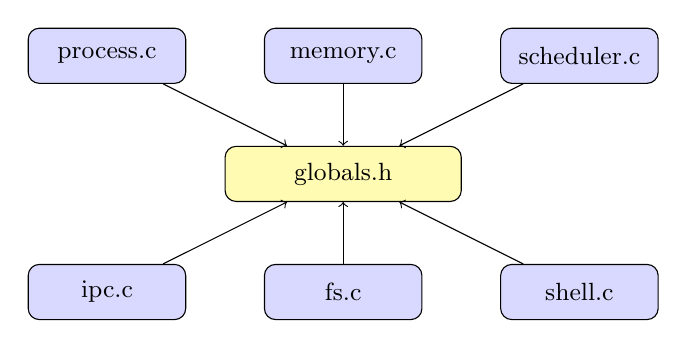
\begin{tikzpicture}[
    module/.style={rectangle, draw, rounded corners, minimum width=2cm, minimum height=0.7cm, fill=blue!15, font=\small}
]
    \node[module, fill=yellow!30, minimum width=3cm] (globals) at (0,0) {globals.h};
    
    \node[module] (process) at (-3,1.5) {process.c};
    \node[module] (memory) at (0,1.5) {memory.c};
    \node[module] (scheduler) at (3,1.5) {scheduler.c};
    \node[module] (ipc) at (-3,-1.5) {ipc.c};
    \node[module] (fs) at (0,-1.5) {fs.c};
    \node[module] (shell) at (3,-1.5) {shell.c};
    
    \draw[->] (process) -- (globals);
    \draw[->] (memory) -- (globals);
    \draw[->] (scheduler) -- (globals);
    \draw[->] (ipc) -- (globals);
    \draw[->] (fs) -- (globals);
    \draw[->] (shell) -- (globals);
    
\end{tikzpicture}
\caption{Modül-Header Bağımlılığı}
\end{figure}

% =============================================================================
% BOLUM 3: SUREC YONETIMI
% =============================================================================
\chapter{Süreç Yönetimi}

\section{Süreç Durumları}

Bir süreç beş farklı durumda olabilir:

\begin{figure}[h]
\centering
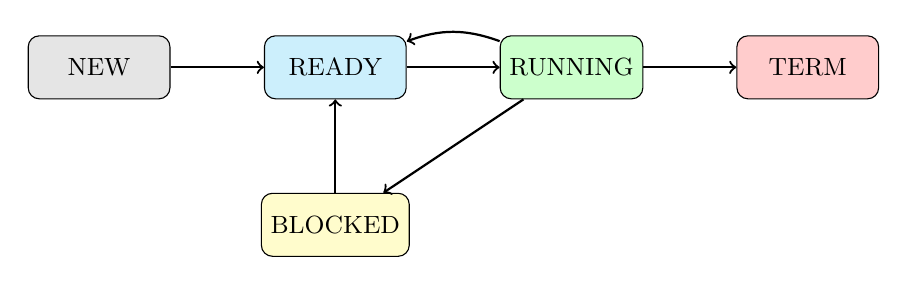
\begin{tikzpicture}[node distance=3cm, auto,
    state/.style={rectangle, draw, rounded corners, minimum width=1.8cm, minimum height=0.8cm, align=center, font=\small}]
    
    \node[state, fill=gray!20] (new) {NEW};
    \node[state, fill=cyan!20, right of=new] (ready) {READY};
    \node[state, fill=green!20, right of=ready] (running) {RUNNING};
    \node[state, fill=yellow!20, below of=ready, node distance=2cm] (blocked) {BLOCKED};
    \node[state, fill=red!20, right of=running] (term) {TERM};
    
    \draw[->, thick] (new) -- (ready);
    \draw[->, thick] (ready) -- (running);
    \draw[->, thick] (running) to[bend right=20] (ready);
    \draw[->, thick] (running) -- (blocked);
    \draw[->, thick] (blocked) -- (ready);
    \draw[->, thick] (running) -- (term);
    
\end{tikzpicture}
\caption{Süreç Durum Geçişleri}
\end{figure}

\begin{itemize}
    \item \textbf{NEW:} Süreç yeni oluşturuldu
    \item \textbf{READY:} Çalışmaya hazır, CPU bekliyor
    \item \textbf{RUNNING:} CPU üzerinde çalışıyor
    \item \textbf{BLOCKED:} I/O işlemi bekliyor
    \item \textbf{TERMINATED:} Çalışma tamamlandı
\end{itemize}

\section{Süreç Kontrol Bloğu (PCB)}

Her süreç için tutulan bilgiler:

\begin{lstlisting}[caption={SimProcess Yapisi}]
typedef struct {
    int pid;                    // Benzersiz surec ID
    char name[32];              // Surec adi
    ProcessState state;         // Mevcut durum
    int priority;               // Oncelik seviyesi (0-9)
    int time_slice;             // Kalan CPU zamani
    
    // Izole Bellek
    int memory_base;            // Baslangic adresi
    int memory_limit;           // Maksimum boyut (4096 byte)
    char memory_space[4096];    // Ozel bellek alani
    int memory_used;            // Kullanilan miktar
    
    // IPC
    IPCMessage mailbox[10];     // Mesaj kutusu
    int mailbox_count;          // Bekleyen mesaj sayisi
    
    bool active;                // Aktif durumu
} SimProcess;
\end{lstlisting}

\section{Surec Olusturma}

\begin{lstlisting}[caption={process\_create Fonksiyonu}]
SimProcess* process_create(char *name, int priority) {
    // Bos slot bul
    for(int i = 0; i < MAX_PROCESS; i++) {
        if(!process_table[i].active) {
            SimProcess *proc = &process_table[i];
            
            // PID ata
            proc->pid = pid_counter++;
            strncpy(proc->name, name, 31);
            proc->state = PROC_READY;
            proc->priority = priority;
            proc->time_slice = 3;
            
            // Izole bellek alani baslat
            proc->memory_base = i * PROCESS_MEMORY_SIZE;
            proc->memory_limit = PROCESS_MEMORY_SIZE;
            memset(proc->memory_space, 0, PROCESS_MEMORY_SIZE);
            
            proc->active = true;
            return proc;
        }
    }
    return NULL;  // Tablo dolu
}
\end{lstlisting}

\section{Surec Sonlandirma}

\begin{lstlisting}[caption={process\_terminate Fonksiyonu}]
void process_terminate(int pid) {
    SimProcess *proc = process_find(pid);
    if(!proc) return;
    
    proc->state = PROC_TERMINATED;
    proc->active = false;
    
    // Guvenlik: Bellegi temizle
    memset(proc->memory_space, 0, PROCESS_MEMORY_SIZE);
}
\end{lstlisting}

% =============================================================================
% BOLUM 4: BELLEK YONETIMI
% =============================================================================
% BOLUM 4: BELLEK YONETIMI
% =============================================================================
\chapter{Bellek Yönetimi}

\section{İzole Bellek Modeli}

Her sürecin 4KB (4096 byte) özel bellek alanı vardır. Süreçler birbirlerinin belleğine erişemez.

\begin{figure}[h]
\centering
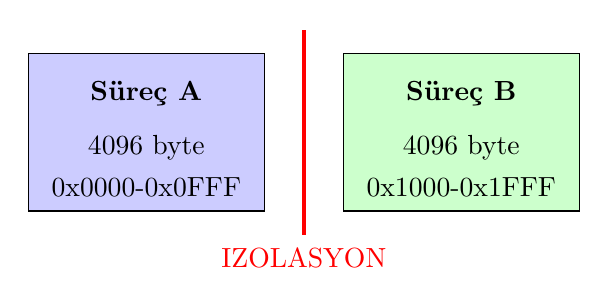
\begin{tikzpicture}
    \draw[fill=blue!20] (0,0) rectangle (3,2);
    \node at (1.5,1.5) {\textbf{Süreç A}};
    \node at (1.5,0.8) {4096 byte};
    \node at (1.5,0.3) {0x0000-0x0FFF};
    
    \draw[fill=green!20] (4,0) rectangle (7,2);
    \node at (5.5,1.5) {\textbf{Süreç B}};
    \node at (5.5,0.8) {4096 byte};
    \node at (5.5,0.3) {0x1000-0x1FFF};
    
    \draw[ultra thick, red] (3.5,-0.3) -- (3.5,2.3);
    \node[red] at (3.5,-0.6) {IZOLASYON};
\end{tikzpicture}
\caption{Bellek İzolasyonu}
\end{figure}

\section{Belleğe Yazma}

\begin{lstlisting}[caption={mem\_write Fonksiyonu}]
int mem_write(int pid, int offset, void *data, int size) {
    SimProcess *proc = process_find(pid);
    if(!proc) return -1;
    
    // Sinir kontrolu
    if(offset < 0 || offset + size > proc->memory_limit) {
        printf("SEGMENTATION FAULT!\n");
        printf("Surec: %s, Offset: %d, Size: %d\n",
               proc->name, offset, size);
        proc->state = PROC_TERMINATED;
        return -1;
    }
    
    // Veriyi yaz
    memcpy(proc->memory_space + offset, data, size);
    
    if(offset + size > proc->memory_used)
        proc->memory_used = offset + size;
    
    return 0;
}
\end{lstlisting}

\section{Bellekten Okuma}

\begin{lstlisting}[caption={mem\_read Fonksiyonu}]
int mem_read(int pid, int offset, void *buffer, int size) {
    SimProcess *proc = process_find(pid);
    if(!proc) return -1;
    
    // Sinir kontrolu
    if(offset < 0 || offset + size > proc->memory_limit) {
        printf("SEGMENTATION FAULT!\n");
        return -1;
    }
    
    memcpy(buffer, proc->memory_space + offset, size);
    return 0;
}
\end{lstlisting}

\section{Neden Sınır Kontrolü?}

Sınır kontrolü \textbf{buffer overflow} saldırılarını önler:

\begin{enumerate}
    \item Hatalı kod kendi alanının dışına yazamaz
    \item Diğer süreçlerin verileri korunur
    \item Güvenlik açıkları önlenir
\end{enumerate}

% =============================================================================
% BOLUM 5: ZAMANLAYICI
% =============================================================================
\chapter{CPU Zamanlayıcısı}

\section{Round-Robin Algoritması}

NexOS, \textbf{Round-Robin} zamanlama algoritması kullanır:

\begin{enumerate}
    \item Her sürece eşit zaman dilimi (quantum) verilir
    \item Zaman dolunca süreç kuyruğa alınır
    \item Sıradaki süreç çalışmaya başlar
    \item Son süreç bitince başa dönülür
\end{enumerate}

\begin{figure}[h]
\centering
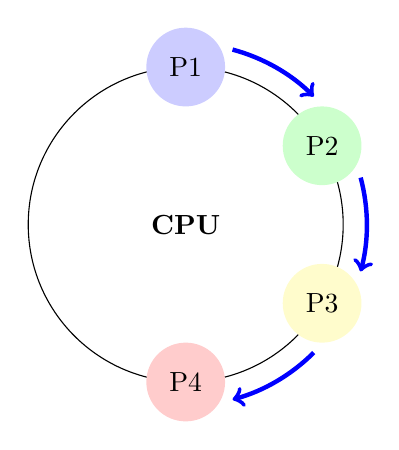
\begin{tikzpicture}
    \draw (0,0) circle (2cm);
    
    \node[fill=blue!20, circle, minimum size=1cm] at (90:2) {P1};
    \node[fill=green!20, circle, minimum size=1cm] at (30:2) {P2};
    \node[fill=yellow!20, circle, minimum size=1cm] at (-30:2) {P3};
    \node[fill=red!20, circle, minimum size=1cm] at (-90:2) {P4};
    
    \draw[->, ultra thick, blue] (75:2.3) arc (75:45:2.3);
    \draw[->, ultra thick, blue] (15:2.3) arc (15:-15:2.3);
    \draw[->, ultra thick, blue] (-45:2.3) arc (-45:-75:2.3);
    
    \node at (0,0) {\textbf{CPU}};
\end{tikzpicture}
\caption{Round-Robin Döngüsü}
\end{figure}

\section{Zaman Dilimi}

\begin{lstlisting}[caption={Zaman Dilimi Tanimi}]
#define TIME_QUANTUM 3  // Her surec 3 tick calisir
\end{lstlisting}

\section{Zamanlayıcı Tick}

\begin{lstlisting}[caption={scheduler\_tick Fonksiyonu}]
void scheduler_tick() {
    scheduler_tick_count++;
    
    // Calisan sureci bul
    SimProcess *current = NULL;
    for(int i = 0; i < MAX_PROCESS; i++) {
        if(process_table[i].state == PROC_RUNNING) {
            current = &process_table[i];
            break;
        }
    }
    
    if(current) {
        current->time_slice--;
        
        if(current->time_slice <= 0) {
            // Zaman doldu - preempt
            current->state = PROC_READY;
            current->time_slice = TIME_QUANTUM;
            
            // Siradaki hazir sureci bul
            int next = find_next_ready();
            if(next >= 0) {
                process_table[next].state = PROC_RUNNING;
            }
        }
    }
}
\end{lstlisting}

% =============================================================================
% BOLUM 6: SURECLER ARASI ILETISIM
% =============================================================================
\chapter{Süreçler Arası İletişim (IPC)}

\section{Mesaj Geçirme Modeli}

Süreçler izole olduğu için doğrudan iletişim kuramaz. NexOS, \textbf{posta kutusu} (mailbox) modeli kullanır.

\begin{figure}[h]
\centering
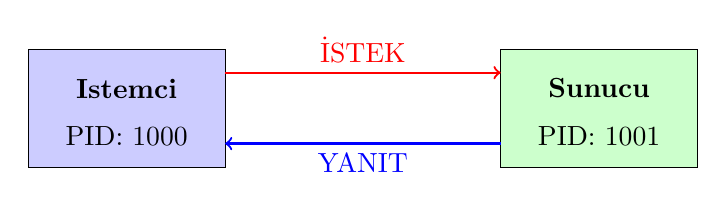
\begin{tikzpicture}
    \draw[fill=blue!20] (0,0) rectangle (2.5,1.5);
    \node at (1.25,1) {\textbf{Istemci}};
    \node at (1.25,0.4) {PID: 1000};
    
    \draw[fill=green!20] (6,0) rectangle (8.5,1.5);
    \node at (7.25,1) {\textbf{Sunucu}};
    \node at (7.25,0.4) {PID: 1001};
    
    \draw[->, thick, red] (2.5,1.2) -- (6,1.2) node[midway, above] {İSTEK};
    \draw[->, thick, blue] (6,0.3) -- (2.5,0.3) node[midway, below] {YANIT};
\end{tikzpicture}
\caption{İstemci-Sunucu Mesajlaşma}
\end{figure}

\section{Mesaj Gönderme}

\begin{lstlisting}[caption={ipc\_send Fonksiyonu}]
int ipc_send(int sender_pid, int receiver_pid, char *message) {
    SimProcess *sender = process_find(sender_pid);
    SimProcess *receiver = process_find(receiver_pid);
    
    if(!sender || !receiver) return -1;
    
    // Alicinin posta kutusunda bos yer bul
    for(int i = 0; i < MAX_IPC_MESSAGES; i++) {
        if(receiver->mailbox[i].read) {
            receiver->mailbox[i].sender_pid = sender_pid;
            strncpy(receiver->mailbox[i].content, message,
                    MAX_IPC_MSG_SIZE - 1);
            receiver->mailbox[i].read = false;
            receiver->mailbox_count++;
            
            // Alici bloklu ise uyandir
            if(receiver->state == PROC_BLOCKED) {
                receiver->state = PROC_READY;
            }
            return 0;
        }
    }
    return -1;  // Kutu dolu
}
\end{lstlisting}

\section{Mesaj Alma}

\begin{lstlisting}[caption={ipc\_receive Fonksiyonu}]
int ipc_receive(int pid, char *buffer) {
    SimProcess *proc = process_find(pid);
    if(!proc) return -1;
    
    // Ilk okunmamis mesaji bul
    for(int i = 0; i < MAX_IPC_MESSAGES; i++) {
        if(!proc->mailbox[i].read) {
            strcpy(buffer, proc->mailbox[i].content);
            proc->mailbox[i].read = true;
            proc->mailbox_count--;
            return 0;
        }
    }
    return -1;  // Mesaj yok
}
\end{lstlisting}

% =============================================================================
% BOLUM 7: DOSYA SISTEMI
% =============================================================================
\chapter{Dosya Sistemi}

\section{Sanal Disk}

NexOS, bir sanal disk kullanır. Dosyalar \texttt{sanal\_disk.bin} dosyasında saklanır.

\begin{lstlisting}[caption={Dosya Blogu Yapisi}]
typedef struct {
    char ad[32];           // Dosya adi
    int boyut;             // Dosya boyutu
    char icerik[1024];     // Dosya icerigi
    bool dolu;             // Kullaniliyor mu?
} DosyaBlogu;

DosyaBlogu sanal_disk[50]; // 50 dosya kapasitesi
\end{lstlisting}

\begin{figure}[h]
\centering
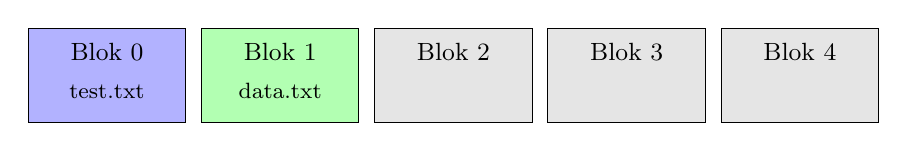
\begin{tikzpicture}
    \foreach \i in {0,...,4} {
        \draw[fill=gray!20] (\i*2.2,0) rectangle (\i*2.2+2,1.2);
        \node at (\i*2.2+1,0.9) {\small Blok \i};
    }
    \draw[fill=blue!30] (0,0) rectangle (2,1.2);
    \node at (1,0.9) {\small Blok 0};
    \node at (1,0.4) {\footnotesize test.txt};
    
    \draw[fill=green!30] (2.2,0) rectangle (4.2,1.2);
    \node at (3.2,0.9) {\small Blok 1};
    \node at (3.2,0.4) {\footnotesize data.txt};
\end{tikzpicture}
\caption{Sanal Disk Blokları}
\end{figure}

\section{Dosya İşlemleri}

\begin{lstlisting}[caption={Dosya Olusturma}]
void sfs_dosya_olustur(char *isim, char *icerik) {
    for(int i = 0; i < MAX_DOSYA; i++) {
        if(!sanal_disk[i].dolu) {
            strncpy(sanal_disk[i].ad, isim, 31);
            strncpy(sanal_disk[i].icerik, icerik,
                    MAX_DOSYA_BOYUTU - 1);
            sanal_disk[i].boyut = strlen(icerik);
            sanal_disk[i].dolu = true;
            sfs_kaydet();
            return;
        }
    }
}
\end{lstlisting}

% =============================================================================
% BOLUM 8: LOG ANALIZ ARACLARI
% =============================================================================
\chapter{Log Analiz Araçları}

\section{Genel Bakış}

NexOS, web sunucuların oluşturduğu log dosyalarını analiz etmek için kapsamlı script araçları içerir. Bu araçlar sistem yöneticilerine:

\begin{itemize}
    \item Ziyaretçi trafiğini anlamak
    \item Güvenlik tehditlerini tespit etmek
    \item Performans sorunlarını belirlemek
    \item Otomatik raporlar oluşturmak
\end{itemize}

imkanı sağlar. Scriptler shell programlama ile yazılmış olup, modüler ve genişletilebilir bir yapıya sahiptir.

\section{Web Sunucu Log Dosyaları}

Web sunucular her isteği bir log dosyasına kaydeder. Bu dosyalar genellikle ``Combined Log Format'' formatında tutulur:

\begin{lstlisting}[style=bashstyle,caption={access.log Ornek Satirlar}]
192.168.1.100 - - [30/Dec/2025:10:15:32 +0300] "GET /index.html HTTP/1.1" 200 4523 "-" "Mozilla/5.0"
192.168.1.101 - - [30/Dec/2025:10:15:45 +0300] "GET /admin.php HTTP/1.1" 404 512 "-" "Chrome/90.0"
10.0.0.50 - - [30/Dec/2025:10:16:01 +0300] "POST /login HTTP/1.1" 401 128 "-" "curl/7.68.0"
\end{lstlisting}

Her satırdaki alanlar:

\begin{tabular}{|c|l|l|}
\hline
\textbf{Alan} & \textbf{Örnek} & \textbf{Anlamı} \\
\hline
\$1 & 192.168.1.100 & Ziyaretçi IP adresi \\
\$4 & [30/Dec/2025:10:15:32] & Tarih ve saat \\
\$6 & GET & HTTP metodu \\
\$7 & /index.html & İstenen sayfa \\
\$9 & 200 & HTTP durum kodu \\
\$10 & 4523 & Gönderilen byte sayısı \\
\hline
\end{tabular}

\section{Modüler Script Yapısı}

Log analiz scripti modüler bir yapıda tasarlanmıştır. Her analiz görevi ayrı bir fonksiyon olarak tanımlanır ve ana program bu fonksiyonları çağırarak rapor oluşturur.

\begin{lstlisting}[style=bashstyle,caption={Script Konfigurasyon Bolumu}]
#!/bin/sh
# NexOS Log Analyzer - Kapsamli Web Log Analiz Araci

# Yapilandirma degiskenleri
LOG_DIR="/var/log/httpd"
ACCESS_LOG="${LOG_DIR}/access.log"
REPORT_DIR="/var/www/reports"
HTML_REPORT="${REPORT_DIR}/index.html"
DATE=$(date +"%Y-%m-%d")
TIME=$(date +"%H:%M:%S")

# Terminal renkleri
RED='\033[0;31m'
GREEN='\033[0;32m'
YELLOW='\033[1;33m'
NC='\033[0m'
\end{lstlisting}

\subsection{Yardımcı Fonksiyonlar}

Tüm modüller tarafından kullanılan ortak fonksiyonlar:

\begin{lstlisting}[style=bashstyle,caption={Yardimci Fonksiyonlar}]
# Bilgi mesaji yazdir
log_info() {
    echo -e "${GREEN}[INFO]${NC} $1"
}

# Uyari mesaji yazdir
log_warn() {
    echo -e "${YELLOW}[WARN]${NC} $1"
}

# Hata mesaji yazdir
log_error() {
    echo -e "${RED}[ERROR]${NC} $1"
}

# Gerekli dizinleri olustur
ensure_directories() {
    # Her dizin icin kontrol yap
    for dir in "$LOG_DIR" "$REPORT_DIR"; do
        # Dizin yoksa olustur
        if [ ! -d "$dir" ]; then
            mkdir -p "$dir"
            log_info "Dizin olusturuldu: $dir"
        fi
    done
}
\end{lstlisting}

\section{Trafik Analizi Fonksiyonları}

\subsection{En Aktif Ziyaretçileri Bulma}

Hangi IP adreslerinden en çok istek geldiğini bulmak için:

\begin{lstlisting}[style=bashstyle,caption={IP Analizi Fonksiyonu}]
get_top_ips() {
    local log_file="$1"
    local count="${2:-10}"  # Varsayilan: 10
    
    # Log dosyasi var mi kontrol et
    if [ ! -f "$log_file" ]; then
        log_error "Log dosyasi bulunamadi: $log_file"
        return 1
    fi
    
    # IP'leri cikart, sirala, say ve en coklari goster
    awk '{print $1}' "$log_file" | \
        sort | \
        uniq -c | \
        sort -rn | \
        head -n "$count"
}
\end{lstlisting}

Bu fonksiyon çalıştığında log dosyasındaki her satırın ilk alanını (IP adresi) alır, bunları sıralar, tekrar edenleri sayar ve en çok tekrar edenleri listeler. Pipe (|) karakteri ile komutlar zincirleme bağlanıyor.

\subsection{En Çok Ziyaret Edilen Sayfalar}

\begin{lstlisting}[style=bashstyle,caption={Sayfa Analizi Fonksiyonu}]
get_top_pages() {
    local log_file="$1"
    local count="${2:-10}"
    
    # 7. sutun sayfa URL'sini icerir
    awk '{print $7}' "$log_file" | \
        grep -v "^-$" | \    # Bos satirlari at
        sort | \
        uniq -c | \
        sort -rn | \
        head -n "$count"
}
\end{lstlisting}

\subsection{HTTP Durum Kodları Dağılımı}

Sunucunun verdiği cevapların dağılımını görmek için:

\begin{lstlisting}[style=bashstyle,caption={Durum Kodu Analizi}]
get_status_codes() {
    local log_file="$1"
    
    # 9. sutun HTTP durum kodunu icerir
    awk '{print $9}' "$log_file" | \
        grep -E "^[0-9]{3}$" | \  # Sadece 3 haneli kodlar
        sort | \
        uniq -c | \
        sort -rn
}
\end{lstlisting}

Durum kodlarının anlamı:
\begin{itemize}
    \item \textbf{200} - Başarılı istek
    \item \textbf{301/302} - Yönlendirme
    \item \textbf{404} - Sayfa bulunamadı
    \item \textbf{500} - Sunucu hatası
\end{itemize}

\subsection{Hata İsteklerini Analiz Etme}

404 ve 500 gibi hataları tespit etmek güvenlik ve bakım için önemlidir:

\begin{lstlisting}[style=bashstyle,caption={Hata Analizi Fonksiyonu}]
get_error_requests() {
    local log_file="$1"
    local count="${2:-20}"
    
    # 4xx ve 5xx kodlarini filtrele
    awk '$9 ~ /^[45][0-9][0-9]$/ {print $9, $7, $1}' "$log_file" | \
        sort | \
        uniq -c | \
        sort -rn | \
        head -n "$count"
}
\end{lstlisting}

Bu fonksiyon sadece hata kodlarını değil, aynı zamanda hangi sayfaların hangi IP'lerden istek aldıktan sonra hata verdiğini de gösterir.

\subsection{Saatlik Trafik Analizi}

Hangi saatlerde daha yoğun trafik olduğunu anlamak için:

\begin{lstlisting}[style=bashstyle,caption={Saatlik Trafik Fonksiyonu}]
get_hourly_traffic() {
    local log_file="$1"
    
    awk '{
        # Zaman damgasindan saat bilgisini cikar
        # Format: [DD/Mon/YYYY:HH:MM:SS
        match($4, /:[0-9]{2}:/, arr)
        if (RSTART > 0) {
            hour = substr($4, RSTART+1, 2)
            hours[hour]++
        }
    }
    END {
        # Sonuclari yazdir
        for (h in hours) {
            printf "%s:00 - %d istek\n", h, hours[h]
        }
    }' "$log_file" | sort
}
\end{lstlisting}

\subsection{Bant Genişliği Hesaplama}

Sunucunun toplam ne kadar veri gönderdiğini hesaplamak için:

\begin{lstlisting}[style=bashstyle,caption={Bant Genisligi Hesaplama}]
get_bandwidth() {
    local log_file="$1"
    
    awk '{
        total += $10  # 10. sutun byte sayisi
    }
    END {
        # Okunabilir formata cevir
        if (total > 1073741824) {
            printf "%.2f GB\n", total/1073741824
        } else if (total > 1048576) {
            printf "%.2f MB\n", total/1048576
        } else if (total > 1024) {
            printf "%.2f KB\n", total/1024
        } else {
            printf "%d bytes\n", total
        }
    }' "$log_file"
}
\end{lstlisting}

\section{Güvenlik Tehdit Tespiti}

Log dosyalarında bilinen saldırı imzalarını aramak için:

\begin{lstlisting}[style=bashstyle,caption={Guvenlik Taramasi}]
detect_threats() {
    local log="$1"
    
    echo "--- GUVENLIK UYARILARI ---"
    
    # Directory Traversal, SQL Injection, XSS tespiti
    if grep -qE "(\.\.\/|etc\/passwd|union select|<script>)" "$log"; then
        echo "[KRITIK] Saldiri girisimi tespit edildi:"
        grep -E "(\.\.\/|etc\/passwd|union select|<script>)" "$log" | head -n 3
    else
        echo "[OK] Bilinen saldiri imzasi bulunamadi."
    fi
    
    # Hassas dosyalara erisim tespiti
    if grep -qE "(admin|login|config|\.env|\.git)" "$log"; then
        echo "[UYARI] Hassas yol erisim girisimi:"
        grep -E "(admin|login|config)" "$log" | head -n 3
    fi
    
    # Brute Force tespiti (cok sayida basarisiz giris)
    local failed_logins=$(grep "401" "$log" | grep "login" | wc -l)
    if [ "$failed_logins" -gt 5 ]; then
        echo "[KRITIK] Brute Force saldirisi olabilir!"
        echo "Basarisiz giris denemesi: $failed_logins"
    fi
}
\end{lstlisting}

\section{Rapor Üretimi}

\subsection{Metin Raporu}

Terminal veya e-posta için metin formatında rapor:

\begin{lstlisting}[style=bashstyle,caption={Metin Rapor Uretimi}]
generate_text_report() {
    local log_file="$1"
    local output_file="${REPORT_DIR}/rapor_${DATE}.txt"
    
    log_info "Metin raporu olusturuluyor..."
    
    {
        echo "=============================================="
        echo "   NEXOS WEB LOG ANALIZ RAPORU"
        echo "=============================================="
        echo "Tarih: ${DATE} ${TIME}"
        echo "Log Dosyasi: ${log_file}"
        echo ""
        
        echo "--- OZET ---"
        echo "Toplam Istek: $(wc -l < "$log_file")"
        echo "Benzersiz Ziyaretci: $(awk '{print $1}' "$log_file" | sort -u | wc -l)"
        echo "Bant Genisligi: $(get_bandwidth "$log_file")"
        echo ""
        
        echo "--- EN COK GELEN IP ADRESLERI ---"
        get_top_ips "$log_file" 10
        echo ""
        
        echo "--- EN COK ZIYARET EDILEN SAYFALAR ---"
        get_top_pages "$log_file" 10
        echo ""
        
        echo "--- HTTP DURUM KODLARI ---"
        get_status_codes "$log_file"
        echo ""
        
        echo "--- HATALI ISTEKLER ---"
        get_error_requests "$log_file" 10
    } > "$output_file"
    
    log_info "Rapor kaydedildi: $output_file"
}
\end{lstlisting}

\subsection{HTML Rapor ve Dashboard}

Web tarayıcıda görülebilen modern bir dashboard:

\begin{lstlisting}[style=bashstyle,caption={HTML Dashboard Uretimi}]
generate_html_report() {
    local log_file="$1"
    
    log_info "HTML raporu olusturuluyor..."
    
    # Istatistikleri hesapla
    local total_requests=$(wc -l < "$log_file")
    local unique_visitors=$(awk '{print $1}' "$log_file" | sort -u | wc -l)
    local bandwidth=$(get_bandwidth "$log_file")
    
    # HTML dosyasini olustur
    cat > "$HTML_REPORT" << EOF
<!DOCTYPE html>
<html>
<head>
    <title>NexOS Log Dashboard</title>
    <meta http-equiv="refresh" content="30">
    <style>
        body { background: #1a1a2e; color: #eee; font-family: sans-serif; }
        .card { background: rgba(255,255,255,0.05); padding: 20px; 
                border-radius: 10px; margin: 10px; }
        .value { font-size: 2em; color: #00ff88; }
        table { width: 100%; border-collapse: collapse; }
        th, td { padding: 10px; border-bottom: 1px solid #333; }
    </style>
</head>
<body>
    <h1>NexOS Trafik Analizi</h1>
    
    <div class="card">
        <h3>Toplam Istek</h3>
        <div class="value">${total_requests}</div>
    </div>
    
    <div class="card">
        <h3>Benzersiz Ziyaretci</h3>
        <div class="value">${unique_visitors}</div>
    </div>
    
    <div class="card">
        <h3>Bant Genisligi</h3>
        <div class="value">${bandwidth}</div>
    </div>
    
    <div class="card">
        <h2>En Cok Gelen IP Adresleri</h2>
        <table>
            <tr><th>Sayi</th><th>IP</th></tr>
EOF
    
    # IP tablosunu ekle
    get_top_ips "$log_file" 10 | while read count ip; do
        echo "<tr><td>${count}</td><td>${ip}</td></tr>" >> "$HTML_REPORT"
    done
    
    echo "</table></div></body></html>" >> "$HTML_REPORT"
    
    log_info "Dashboard kaydedildi: $HTML_REPORT"
}
\end{lstlisting}

Dashboard her 30 saniyede otomatik yenilenir (meta refresh).

\section{Cron ile Otomatik Zamanlama}

Raporların düzensiz aralıklarda otomatik oluşturulması için cron kullanılır:

\begin{lstlisting}[style=bashstyle,caption={Cron Kurulumu}]
setup_cron() {
    local interval="${1:-hourly}"
    local script_path=$(readlink -f "$0")
    local cron_entry=""
    
    # Araloga gore cron ifadesi olustur
    case "$interval" in
        hourly)
            # Her saat basinda calistir
            cron_entry="0 * * * * $script_path --auto"
            ;;
        daily)
            # Her gun gece yarisi calistir
            cron_entry="0 0 * * * $script_path --auto"
            ;;
        weekly)
            # Her pazar gece yarisi calistir
            cron_entry="0 0 * * 0 $script_path --auto"
            ;;
        *)
            log_error "Bilinmeyen aralik: $interval"
            log_info "Kullanim: hourly, daily, weekly"
            return 1
            ;;
    esac
    
    # Crontab'a ekle (varsa ekleme)
    if crontab -l 2>/dev/null | grep -q "$script_path"; then
        log_warn "Bu script icin cron gorevi zaten mevcut"
    else
        (crontab -l 2>/dev/null; echo "$cron_entry") | crontab -
        log_info "Cron gorevi eklendi: $cron_entry"
    fi
}
\end{lstlisting}

\subsection{Cron İfade Formatı}

\begin{lstlisting}[style=bashstyle]
# Cron formati: dakika saat gun ay haftanin_gunu komut
# Ornekler:
0 * * * *     # Her saat basinda
0 0 * * *     # Her gun gece yarisi
0 0 * * 0     # Her pazar gece yarisi
*/5 * * * *   # Her 5 dakikada bir
0 8,18 * * *  # Her gun saat 8 ve 18'de
\end{lstlisting}

\section{Canlı İzleme Modu}

Sistem yöneticileri log dosyasını canlı olarak izleyebilir:

\begin{lstlisting}[style=bashstyle,caption={Canli Izleme Fonksiyonu}]
live_monitor() {
    local log_file="$1"
    
    log_info "Canli izleme baslatiliyor (Ctrl+C ile durdur)..."
    
    # Sonsuz dongu ile surekli guncelle
    while true; do
        clear
        echo "========================================"
        echo "   NEXOS CANLI LOG MONITOR"
        echo "========================================"
        echo "Zaman: $(date)"
        echo "Log: $log_file"
        echo ""
        
        echo "--- ANLIK ISTATISTIKLER ---"
        echo "Toplam Istek: $(wc -l < "$log_file")"
        echo "Benzersiz Ziyaretci: $(awk '{print $1}' "$log_file" | sort -u | wc -l)"
        echo ""
        
        echo "--- SON 10 ISTEK ---"
        tail -10 "$log_file"
        echo ""
        
        echo "--- EN AKTIF 5 IP ---"
        get_top_ips "$log_file" 5
        
        # 5 saniye bekle ve tekrar et
        sleep 5
    done
}
\end{lstlisting}

Bu mod açık kaldığı sürece ekran her 5 saniyede güncellenir ve sistem yöneticisi anlık trafiği görebilir.

\section{Ana Program Akışı}

Tüm fonksiyonlar tanımlandıktan sonra ana program kullanıcıdan gelen parametrelere göre çalışır:

\begin{lstlisting}[style=bashstyle,caption={Ana Program}]
main() {
    # Dizinleri hazirla
    ensure_directories
    
    local log_file="$ACCESS_LOG"
    local action="all"
    
    # Komut satiri parametrelerini isle
    while [ $# -gt 0 ]; do
        case "$1" in
            --log)
                log_file="$2"
                shift 2
                ;;
            --text)
                action="text"
                shift
                ;;
            --html)
                action="html"
                shift
                ;;
            --setup-cron)
                setup_cron "$2"
                exit 0
                ;;
            --live)
                live_monitor "$log_file"
                exit 0
                ;;
            --help)
                show_help
                exit 0
                ;;
            *)
                log_error "Bilinmeyen parametre: $1"
                exit 1
                ;;
        esac
    done
    
    # Secilen islemi calistir
    case "$action" in
        text)
            generate_text_report "$log_file"
            ;;
        html)
            generate_html_report "$log_file"
            ;;
        all)
            generate_text_report "$log_file"
            generate_html_report "$log_file"
            detect_threats "$log_file"
            ;;
    esac
    
    log_info "Analiz tamamlandi!"
}

# Programi calistir
main "$@"
\end{lstlisting}

\section{Kullanım Örnekleri}

\begin{lstlisting}[style=bashstyle,caption={Script Kullanim Ornekleri}]
# Tam analiz (metin + HTML + guvenlik)
./log_analyzer.sh

# Sadece HTML rapor olustur
./log_analyzer.sh --html

# Farkli bir log dosyasini analiz et
./log_analyzer.sh --log /var/log/nginx/access.log

# Canli izleme baslat
./log_analyzer.sh --live

# Gunluk otomatik rapor icin cron kur
./log_analyzer.sh --setup-cron daily

# Haftalik otomatik rapor icin cron kur
./log_analyzer.sh --setup-cron weekly

# En cok istekte bulunan 20 IP'yi goster
./log_analyzer.sh --top-ips 20
\end{lstlisting}

% =============================================================================
% BOLUM 9: YAPAY ZEKA ENTEGRASYONU
% =============================================================================
\chapter{Yapay Zeka Entegrasyonu}

\section{Genel Bakış}

NexOS, kullanıcılara komut önerilerinde bulunmak ve sistem yönetimini kolaylaştırmak için entegre bir yapay zeka asistanı içerir. Bu asistan:

\begin{itemize}
    \item Ollama AI çalışma zamanını kullanır
    \item Özel eğitilmiş ``nexos-expert'' modelini çalıştırır
    \item Kullanıcı sorularını analiz ederek BusyBox komutları önerir
    \item Tehlikeli komutları filtreleyerek güvenlik sağlar
\end{itemize}

\section{Ollama AI Motoru}

Ollama, yerel olarak çalışan ve çeşitli dil modellerini destekleyen açık kaynak bir AI çalışma zamanıdır. NexOS'ta Ollama sunucu modu ile çalışır:

\begin{lstlisting}[style=bashstyle,caption={Ollama Sunucu Baslatma}]
# Ollama sunucusunu arka planda baslat
/bin/ollama serve > /var/log/ollama.log 2>&1 &

# Sunucunun hazir olmasini bekle
for i in 1 2 3 4 5 6 7 8 9 10; do
    sleep 2
    if wget -q -O /dev/null http://127.0.0.1:11434/api/tags; then
        echo "Ollama hazir!"
        break
    fi
    echo "Bekleniyor... ($i/10)"
done
\end{lstlisting}

\section{Özel Model Oluşturma}

NexOS, GGUF formatında bir model dosyası ve Modelfile kullanarak özel bir AI modeli oluşturur:

\begin{lstlisting}[style=bashstyle,caption={Modelfile Icerigi}]
# /root/Modelfile
FROM /root/nexos-expert.gguf

PARAMETER temperature 0.1
PARAMETER top_p 0.9

SYSTEM "You are NexOS Assistant, a specialized AI for a custom 
Linux distro. You ONLY output BusyBox commands in the format: 
COMMAND: <cmd>
EXPLANATION: <text>
You are helpful, safe, and concise."
\end{lstlisting}

\begin{lstlisting}[style=bashstyle,caption={Model Kayit Islemi}]
# Modeli Ollama'ya kaydet
/bin/ollama create nexos-expert -f /root/Modelfile

# Kayitli modelleri listele
/bin/ollama list
\end{lstlisting}

\section{AI Modülü (ai.c)}

C kodunda AI entegrasyonu şu şekilde yapılır:

\begin{lstlisting}[caption={AI Model Kontrolu}]
void ensure_ai_model_exists() {
    if (ai_model_ready) return;  // Zaten kontrol edildi
    
    // Ollama binary var mi?
    if (access("/bin/ollama", F_OK) != 0) {
        printf("[AI] Ollama kurulu degil!\n");
        return;
    }
    
    // Modelfile var mi? Yoksa olustur
    if (access("/root/Modelfile", F_OK) != 0) {
        printf("[AI] Modelfile bulunamadi, olusturuluyor...\n");
        
        FILE *f = fopen("/root/Modelfile", "w");
        if (f) {
            fprintf(f, "FROM /root/nexos-expert.gguf\n\n");
            fprintf(f, "PARAMETER temperature 0.1\n");
            fprintf(f, "PARAMETER top_p 0.9\n\n");
            fprintf(f, "SYSTEM \"You are NexOS Assistant...\"\n");
            fclose(f);
        }
    }
    
    // Model kayitli mi kontrol et
    FILE *check = popen("/bin/ollama list | grep nexos-expert", "r");
    if (check) {
        char buf[16] = "";
        if (fgets(buf, sizeof(buf), check) == NULL) {
            // Model kayitli degil, kaydet
            printf("[AI] Model kaydediliyor...\n");
            system("/bin/ollama create nexos-expert -f /root/Modelfile");
        }
        pclose(check);
    }
    
    ai_model_ready = true;
}
\end{lstlisting}

\section{Kullanıcıdan Soru Alma}

\begin{lstlisting}[caption={AI Soru Fonksiyonu}]
void ai_sor(char *soru) {
    char komut[512];
    char tampon[256];
    
    ensure_ai_model_exists();
    
    if (access("/bin/ollama", F_OK) != 0) {
        printf("[HATA] AI Modulu bulunamadi!\n");
        return;
    }

    printf("[AI] NexOS Expert dusuniyor...\n");
    
    sprintf(komut, "/bin/ollama run nexos-expert \"%s\" 2>&1", soru);
    FILE *pipe = popen(komut, "r");
    if (!pipe) {
        perror("popen");
        return;
    }
    
    printf("--- AI Yaniti ---\n");
    while (fgets(tampon, sizeof(tampon), pipe) != NULL) {
        printf("%s", tampon);
    }
    printf("\n-----------------\n");
    
    pclose(pipe);
}
\end{lstlisting}

\section{Komut Öneri ve Çalıştırma}

AI asistanı, kullanıcının sorusuna göre komut önerir ve güvenlik kontrolü sonrası çalıştırır:

\begin{lstlisting}[caption={Komut Guvenlik Kontrolu}]
// Izin verilen komutlar (whitelist)
static const char* ALLOWED_COMMANDS[] = {
    "ls", "cat", "grep", "find", "du", "df",
    "free", "top", "ps", "uptime", "whoami",
    "date", "cal", "pwd", "head", "tail",
    "wc", "sort", "uniq", "awk", "cut",
    NULL
};

bool is_command_safe(const char* cmd) {
    // Tehlikeli karakterleri kontrol et
    if (strstr(cmd, ";") || strstr(cmd, "|") ||
        strstr(cmd, "&") || strstr(cmd, ">") ||
        strstr(cmd, "<") || strstr(cmd, "`") ||
        strstr(cmd, "$")) {
        return false;
    }
    
    // Whitelist kontrolu
    for (int i = 0; ALLOWED_COMMANDS[i] != NULL; i++) {
        if (strncmp(cmd, ALLOWED_COMMANDS[i], 
                    strlen(ALLOWED_COMMANDS[i])) == 0) {
            return true;
        }
    }
    
    return false;
}
\end{lstlisting}

\begin{lstlisting}[caption={AI Komut Yardimcisi}]
void ai_command_helper_run(char *soru) {
    char response[4096];
    char *cmd_start, *cmd_end;
    
    // AI'dan yanit al
    // ... (ollama calistir, response'a yaz)
    
    // "COMMAND:" satirini bul
    cmd_start = strstr(response, "COMMAND:");
    if (cmd_start) {
        cmd_start += 9;  // "COMMAND: " atla
        
        // Satir sonunu bul
        cmd_end = strchr(cmd_start, '\n');
        if (cmd_end) *cmd_end = '\0';
        
        // Bosluklari temizle
        while (*cmd_start == ' ') cmd_start++;
        
        printf("[AI] Onerilen komut: %s\n", cmd_start);
        
        // Guvenlik kontrolu
        if (is_command_safe(cmd_start)) {
            printf("[AI] Komut guvenli, calistiriliyor...\n");
            system(cmd_start);
        } else {
            printf("[AI] UYARI: Komut guvenlik kontrolunu gecemedi!\n");
            printf("Komut manuel olarak calistirilamaz.\n");
        }
    }
}
\end{lstlisting}

\section{AI Modu Kullanim}

NexOS'ta AI modunu kullanmak icin ana menudan ``AI OS Mode'' secilir:

\begin{lstlisting}[style=bashstyle,caption={AI Modu Ornekleri}]
[AI Mode]
Soru: Diskteki en buyuk dosyalari bul
[AI] COMMAND: du -sh /* | sort -rh | head -10
[AI] EXPLANATION: Kok dizindeki en buyuk dosya ve 
     klasorleri boyutuna gore siralar.

Soru: Sistem bellek kullanimini goster
[AI] COMMAND: free -h
[AI] EXPLANATION: RAM ve swap kullanimini 
     okunabilir formatta gosterir.
\end{lstlisting}

% =============================================================================
% BOLUM 10: WEB SUNUCU
% =============================================================================
\chapter{Entegre Web Sunucu}

\section{Genel Bakis}

NexOS, BusyBox httpd tabanli tam ozellikli bir web sunucu icerir. Bu sunucu:

\begin{itemize}
    \item Statik HTML/CSS/JS dosyalari sunar
    \item access.log dosyasi olusturur (log analizi icin)
    \item Temel HTTP kimlik dogrulama (Basic Auth) destekler
    \item Dinamik rapor sayfalarini icerir
\end{itemize}

\section{Web Sunucu Scripti}

\begin{lstlisting}[style=bashstyle,caption={webserver.sh - Konfigurasyon}]
#!/bin/sh
# NexOS Public Web Server Setup

# Konfigurasyon degiskenleri
WEB_ROOT="${WEB_ROOT:-/var/www}"
LOG_DIR="${LOG_DIR:-/var/log/httpd}"
ACCESS_LOG="${LOG_DIR}/access.log"
CONFIG_FILE="${CONFIG_FILE:-/etc/httpd.conf}"
PORT="${PORT:-80}"

# Terminal renkleri
RED='\033[0;31m'
GREEN='\033[0;32m'
YELLOW='\033[1;33m'
NC='\033[0m'

log_info() { echo -e "${GREEN}[INFO]${NC} $1"; }
log_warn() { echo -e "${YELLOW}[WARN]${NC} $1"; }
log_error() { echo -e "${RED}[ERROR]${NC} $1"; }
\end{lstlisting}

\section{Dizin Yapisi Kurulumu}

\begin{lstlisting}[style=bashstyle,caption={Dizin Olusturma}]
setup_directories() {
    log_info "Dizinler hazirlaniyor..."
    
    # Web dizinlerini olustur
    mkdir -p "$WEB_ROOT"/{css,js,images,reports}
    mkdir -p "$LOG_DIR"
    
    # Log dosyasini olustur
    touch "$ACCESS_LOG"
    chmod 644 "$ACCESS_LOG"
    
    # Log dosyasini web dizinine bagla (erisim icin)
    ln -sf "$ACCESS_LOG" "$WEB_ROOT/access.log"
}
\end{lstlisting}

\section{Web Sayfasi Olusturma}

\begin{lstlisting}[style=bashstyle,caption={Ana Sayfa (index.html)}]
create_website() {
    log_info "Web sayfasi olusturuluyor..."
    
    cat > "${WEB_ROOT}/index.html" << 'EOF'
<!DOCTYPE html>
<html>
<head>
    <title>NexOS Web Server</title>
    <style>
        body {
            font-family: 'Segoe UI', sans-serif;
            background: linear-gradient(135deg, #667eea, #764ba2);
            min-height: 100vh;
            display: flex;
            justify-content: center;
            align-items: center;
            color: white;
        }
        .container {
            text-align: center;
            padding: 40px;
            background: rgba(255,255,255,0.1);
            border-radius: 20px;
            backdrop-filter: blur(10px);
        }
        h1 { font-size: 3em; }
        .status {
            background: #00ff88;
            color: #1a1a2e;
            padding: 10px 30px;
            border-radius: 50px;
            display: inline-block;
            font-weight: bold;
        }
        .links a {
            color: white;
            text-decoration: none;
            padding: 12px 25px;
            margin: 5px;
            background: rgba(255,255,255,0.2);
            border-radius: 10px;
            display: inline-block;
        }
        .links a:hover {
            background: rgba(255,255,255,0.4);
        }
    </style>
</head>
<body>
    <div class="container">
        <h1>NexOS Server</h1>
        <div class="status">ONLINE</div>
        <p>Welcome to NexOS Public Web Server</p>
        
        <div class="links">
            <a href="/reports/">Analytics Dashboard</a>
            <a href="/about.html">About</a>
            <a href="/access.log">Access Log</a>
        </div>
    </div>
</body>
</html>
EOF
}
\end{lstlisting}

\section{HTTP Kimlik Dogrulama}

Hassas sayfalara erisimi kisitlamak icin Basic Authentication kullanilir:

\begin{lstlisting}[style=bashstyle,caption={Kimlik Dogrulama Kurulumu}]
setup_authentication() {
    log_info "Kimlik dogrulama ayarlaniyor..."
    
    # Admin icin sifre dosyasi olustur
    # Format: kullanici:sifre
    echo "admin:nexos123" > "${WEB_ROOT}/.htpasswd"
    chmod 600 "${WEB_ROOT}/.htpasswd"
    
    # httpd konfigurasyon dosyasini guncelle
    cat >> "$CONFIG_FILE" << EOF
# Korunmus dizinler
A:admin
/admin
/reports
EOF
    
    log_info "Admin kullanici: admin, Sifre: nexos123"
}
\end{lstlisting}

\section{Sunucu Baslatma ve Durdurma}

\begin{lstlisting}[style=bashstyle,caption={Sunucu Kontrolu}]
start_server() {
    log_info "Web sunucu baslatiliyor..."
    
    # Dizinleri hazirla
    setup_directories
    create_website
    
    # Onceki sureci durdur (varsa)
    pkill -f "httpd.*${WEB_ROOT}" 2>/dev/null
    
    # BusyBox httpd'yi baslat
    busybox httpd -p 0.0.0.0:${PORT} -h "$WEB_ROOT" -f -vv \
        >> "$ACCESS_LOG" 2>&1 &
    
    # PID'i kaydet
    echo $! > /var/run/httpd.pid
    
    log_info "Sunucu baslatildi: http://localhost:${PORT}"
}

stop_server() {
    log_info "Web sunucu durduruluyor..."
    
    if [ -f /var/run/httpd.pid ]; then
        kill $(cat /var/run/httpd.pid) 2>/dev/null
        rm /var/run/httpd.pid
        log_info "Sunucu durduruldu."
    else
        pkill -f "httpd.*${WEB_ROOT}" 2>/dev/null
    fi
}

server_status() {
    if pgrep -f "httpd.*${WEB_ROOT}" > /dev/null; then
        echo -e "${GREEN}Web sunucu CALISIYOR${NC}"
        echo "Port: ${PORT}"
        echo "Log: $(wc -l < "$ACCESS_LOG") satir"
    else
        echo -e "${RED}Web sunucu DURMUS${NC}"
    fi
}
\end{lstlisting}

\section{Canli Log Takibi}

\begin{lstlisting}[style=bashstyle,caption={Log Izleme}]
tail_logs() {
    log_info "Canli log izleme (Ctrl+C ile cik)..."
    tail -f "$ACCESS_LOG"
}
\end{lstlisting}

\section{Ana Program}

\begin{lstlisting}[style=bashstyle,caption={webserver.sh Kullanim}]
# Kullanim ornekleri
./webserver.sh start      # Sunucuyu baslat
./webserver.sh stop       # Sunucuyu durdur
./webserver.sh restart    # Yeniden baslat
./webserver.sh status     # Durum goster
./webserver.sh logs       # Canli log izleme
\end{lstlisting}

% =============================================================================
% BOLUM 11: ISO VE BOOT SURECI
% =============================================================================
\chapter{ISO Oluşturma ve Boot Süreci}

\section{Genel Bakış}

NexOS, bootable bir ISO dosyası olarak dağıtılır. Bu ISO, QEMU veya VirtualBox gibi sanal makinelerde çalıştırılır. ISO oluşturma süreci şu adımları içerir:

\begin{enumerate}
    \item C kodlarının statik derlenmesi
    \item Root dosya sisteminin hazırlanması
    \item BusyBox ve Ollama'nın eklenmesi
    \item Init scriptinin oluşturulması
    \item Initramfs ve ISO imajının üretilmesi
\end{enumerate}

\section{Derleme Süreci}

\begin{lstlisting}[style=bashstyle,caption={Statik Derleme}]
# Makefile'dan
CC = gcc
CFLAGS = -Wall -Wextra -static -O2

# Tum kaynak dosyalarini derle
nexos: main.o process.o memory.o scheduler.o ipc.o fs.o \
       shell.o tui.o hardware.o utils.o ai.o
    $(CC) $(CFLAGS) -o $@ $^

# -static: Tum kutuphaneleri icine al
# Sonuc: Bagimsiz calisabilen tek binary
\end{lstlisting}

\section{Root Dosya Sistemi}
\begin{lstlisting}[style=bashstyle,caption={RootFS Yapisi}]
rootfs/
+-- bin/
|   +-- nexos          # Ana program
|   +-- busybox        # Tum Unix komutlari
|   +-- ollama         # AI motoru
+-- etc/
|   +-- passwd         # Kullanici bilgileri
|   +-- udhcp.script   # DHCP yapilandirmasi
+-- lib/
|   +-- modules/       # Kernel modulleri (e1000.ko)
+-- root/
|   +-- Modelfile      # AI model tanimlama
|   +-- nexos-expert.gguf  # AI model dosyasi
+-- opt/
|   +-- nexos/         # Ek scriptler
+-- var/
    +-- www/           # Web sunucu dizini
    +-- log/           # Log dosyalari
\end{lstlisting}

\section{Init Script}

Kernel başladıktan sonra ilk çalışan script:

\begin{lstlisting}[style=bashstyle,caption={/init - Boot Scripti}]
#!/bin/sh

# 1. Temel dosya sistemlerini bagla
mount -t proc none /proc
mount -t sysfs none /sys
mount -t devtmpfs none /dev
mkdir -p /dev/pts
mount -t devpts devpts /dev/pts

# 2. Ortam degiskenlerini ayarla
export PATH=/bin:/usr/bin:/sbin
export HOME=/root
export TERM=linux

# 3. BusyBox komutlarini kur
busybox --install -s /bin

# 4. Karsilama mesaji
echo "--------------------------------"
echo "   NexOS Live System Booting   "
echo "--------------------------------"

# 5. Ag baglantisini baslat
echo "Starting Networking..."

# VirtualBox/QEMU ag suruculerini yukle
if [ -f /lib/modules/e1000.ko ]; then
    insmod /lib/modules/e1000.ko
fi

# Ag arayuzunu bul ve DHCP ile yapilandir
for iface in $(ls /sys/class/net/ | grep -v lo); do
    ip link set $iface up
    udhcpc -b -i $iface -s /etc/udhcp.script &
done

# 6. Ollama AI servisini baslat
echo "Starting AI Engine..."
mkdir -p /root/.ollama
nohup /bin/ollama serve > /var/log/ollama.log 2>&1 &

# Ollama'nin hazir olmasini bekle
for i in 1 2 3 4 5; do
    sleep 2
    if wget -q -O /dev/null http://127.0.0.1:11434/api/tags; then
        echo "Ollama hazir!"
        break
    fi
done

# 7. AI modelini olustur
if [ -f /root/Modelfile ]; then
    /bin/ollama create nexos-expert -f /root/Modelfile
fi

# 8. Ana programi sonsuz dongude calistir
echo "Starting NexOS..."
while true; do
    /bin/nexos
    echo "NexOS kapandi. Yeniden baslatiliyor..."
    sleep 2
done
\end{lstlisting}

\section{Initramfs Oluşturma}

\begin{lstlisting}[style=bashstyle,caption={Initramfs Paketleme}]
# rootfs dizininden initramfs olustur
cd rootfs
find . | cpio -H newc -o | gzip > ../initramfs.cpio.gz

# Sonuc: ~50-100MB sikistirilmis dosya sistemi
\end{lstlisting}

\section{ISO İmajı Oluşturma}

\begin{lstlisting}[style=bashstyle,caption={ISO Olusturma}]
# ISO dizin yapisi
iso/
+-- boot/
|   +-- isolinux/
|   |   +-- isolinux.bin    # Bootloader
|   |   +-- isolinux.cfg    # Boot konfigurasyonu
|   |   +-- ldlinux.c32     # Gerekli modul
|   +-- vmlinuz             # Linux kernel
|   +-- initramfs.cpio.gz   # Root dosya sistemi
+-- NexOS

# Boot konfigurasyonu (isolinux.cfg)
DEFAULT nexos
LABEL nexos
    KERNEL /boot/vmlinuz
    APPEND initrd=/boot/initramfs.cpio.gz

# ISO olusturma komutu
xorriso -as mkisofs \
    -o nexos.iso \
    -b boot/isolinux/isolinux.bin \
    -c boot/isolinux/boot.cat \
    -no-emul-boot \
    -boot-load-size 4 \
    -boot-info-table \
    -isohybrid-mbr /usr/lib/ISOLINUX/isohdpfx.bin \
    iso/
\end{lstlisting}

\section{ISO Çalıştırma}

\begin{lstlisting}[style=bashstyle,caption={QEMU ile Test}]
# Temel calistirma
qemu-system-x86_64 -cdrom nexos.iso -m 2G

# KVM hizlandirmasi ile (Linux)
qemu-system-x86_64 -cdrom nexos.iso -m 2G -enable-kvm

# Ag ile
qemu-system-x86_64 -cdrom nexos.iso -m 2G \
    -nic user,hostfwd=tcp::8080-:80
\end{lstlisting}

% =============================================================================
% BOLUM 12: KULLANICI ARAYUZU
% =============================================================================
\chapter{Kullanıcı Arayüzü}

\section{Giriş Ekranı}

NexOS başladığında kullanıcı adı ve şifre istenir:

\begin{itemize}
    \item Varsayılan kullanıcı: \texttt{admin}
    \item Varsayılan şifre: \texttt{123}
\end{itemize}

\section{Ana Menü}

Giriş başarılı olunca TUI menüsü gösterilir:

\begin{enumerate}
    \item AI OS Mode - Yapay zeka destekli mod
    \item Manual Mode - Uzman kabuğu
    \item System Information - Sistem bilgisi
    \item Web Server Control - Web sunucu yönetimi
    \item Tools - Araçlar
    \item Power Off - Kapat
\end{enumerate}

\section{Shell Komutları}

\begin{tabular}{|l|l|}
\hline
\textbf{Komut} & \textbf{Açıklama} \\
\hline
\texttt{help} & Tüm komutları listele \\
\texttt{proclist} & Süreç tablosunu göster \\
\texttt{newproc <ad>} & Yeni süreç oluştur \\
\texttt{memdemo} & Bellek izolasyonu demo \\
\texttt{scheddemo} & Zamanlayıcı demo \\
\texttt{ipcdemo} & IPC demo \\
\texttt{analyze <dosya>} & Log dosyası analizi \\
\texttt{traffic} & Trafik analizi \\
\texttt{web} & Web sunucu başlat \\
\texttt{exit} & Çıkış \\
\hline
\end{tabular}

% =============================================================================
% BOLUM 13: SONUC
% =============================================================================
\chapter{Sonuç}

\section{Özellik Özeti}

NexOS aşağıdaki işletim sistemi kavramlarını içerir:

\begin{itemize}
    \item \textbf{Süreç Yönetimi:} Oluşturma, sonlandırma, durum geçişleri
    \item \textbf{Bellek İzolasyonu:} Her süreç için güvenli ayrı alan
    \item \textbf{CPU Zamanlama:} Round-Robin algoritması
    \item \textbf{IPC:} Mesaj tabanlı süreçler arası iletişim
    \item \textbf{Dosya Sistemi:} Kalıcı sanal disk
    \item \textbf{Log Analizi:} awk/sort/uniq ile modüler shell programlama
    \item \textbf{AI Entegrasyonu:} Ollama tabanlı komut asistanı
    \item \textbf{Web Sunucu:} BusyBox httpd ile HTTP sunumu
    \item \textbf{Boot Süreci:} Initramfs ve ISO oluşturma
\end{itemize}

\section{Öğrenilen Kavramlar}

\begin{enumerate}
    \item C ile sistem programlama
    \item Süreç ve bellek yönetimi
    \item Zamanlama algoritmaları
    \item Süreçler arası iletişim
    \item Log dosyası analizi
    \item Bootable ISO oluşturma
\end{enumerate}

% =============================================================================
% EKLER
% =============================================================================
\chapter{Ekler}

\section{Ekran Görüntüleri}

\subsection{Giriş Ekranı}
\begin{center}
    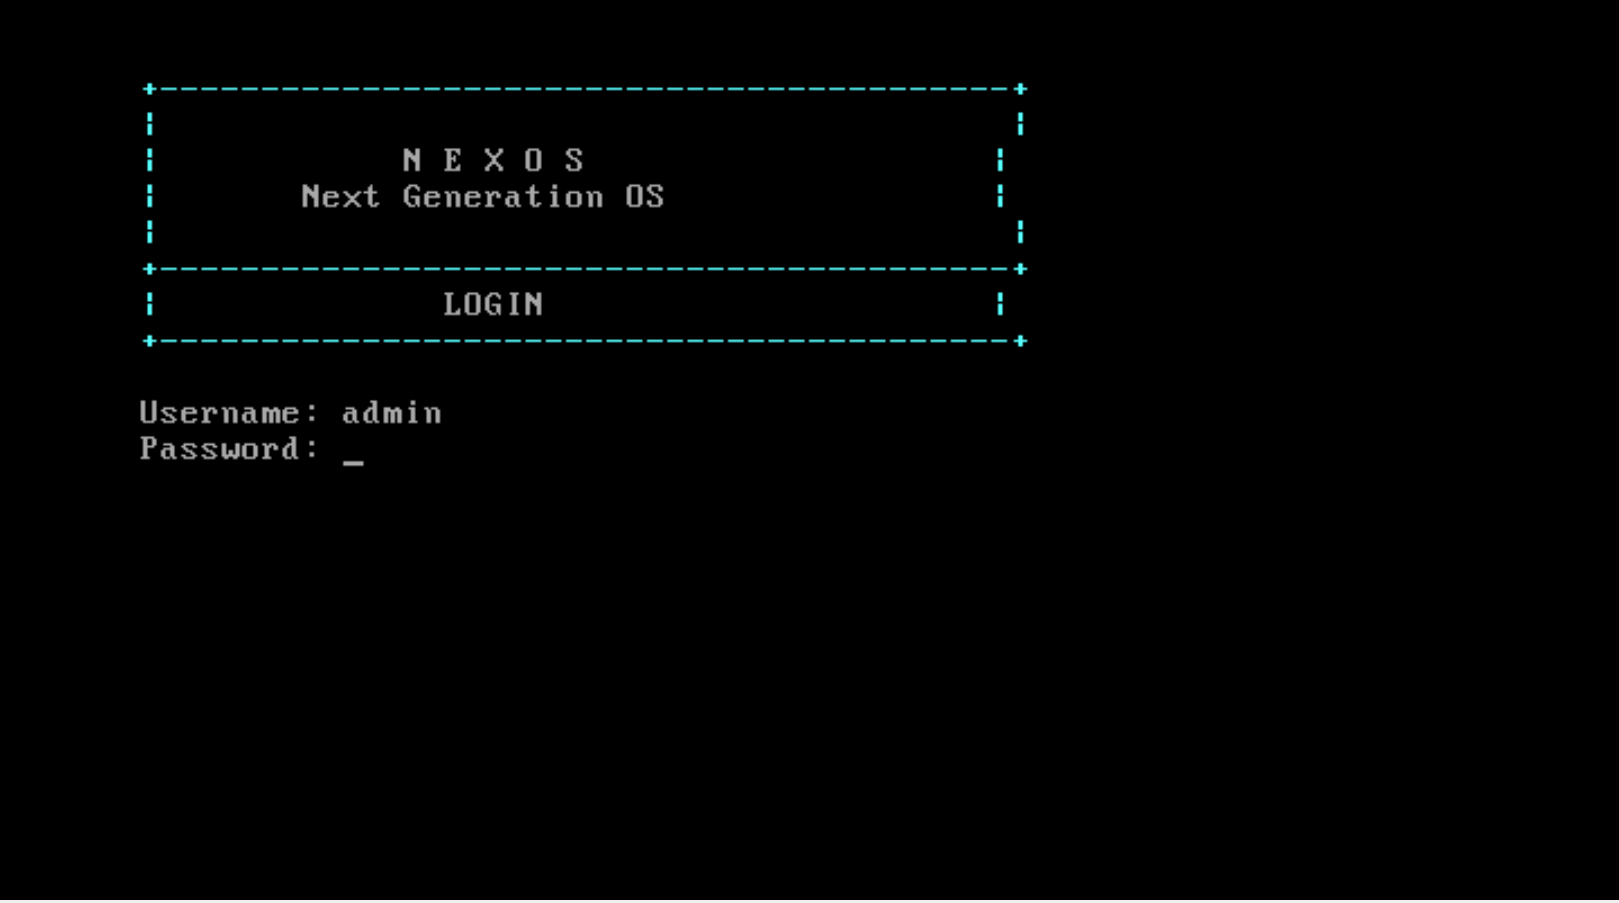
\includegraphics[width=0.8\textwidth]{images/giris.PNG}
\end{center}

\subsection{Ana Ekran}
\begin{center}
    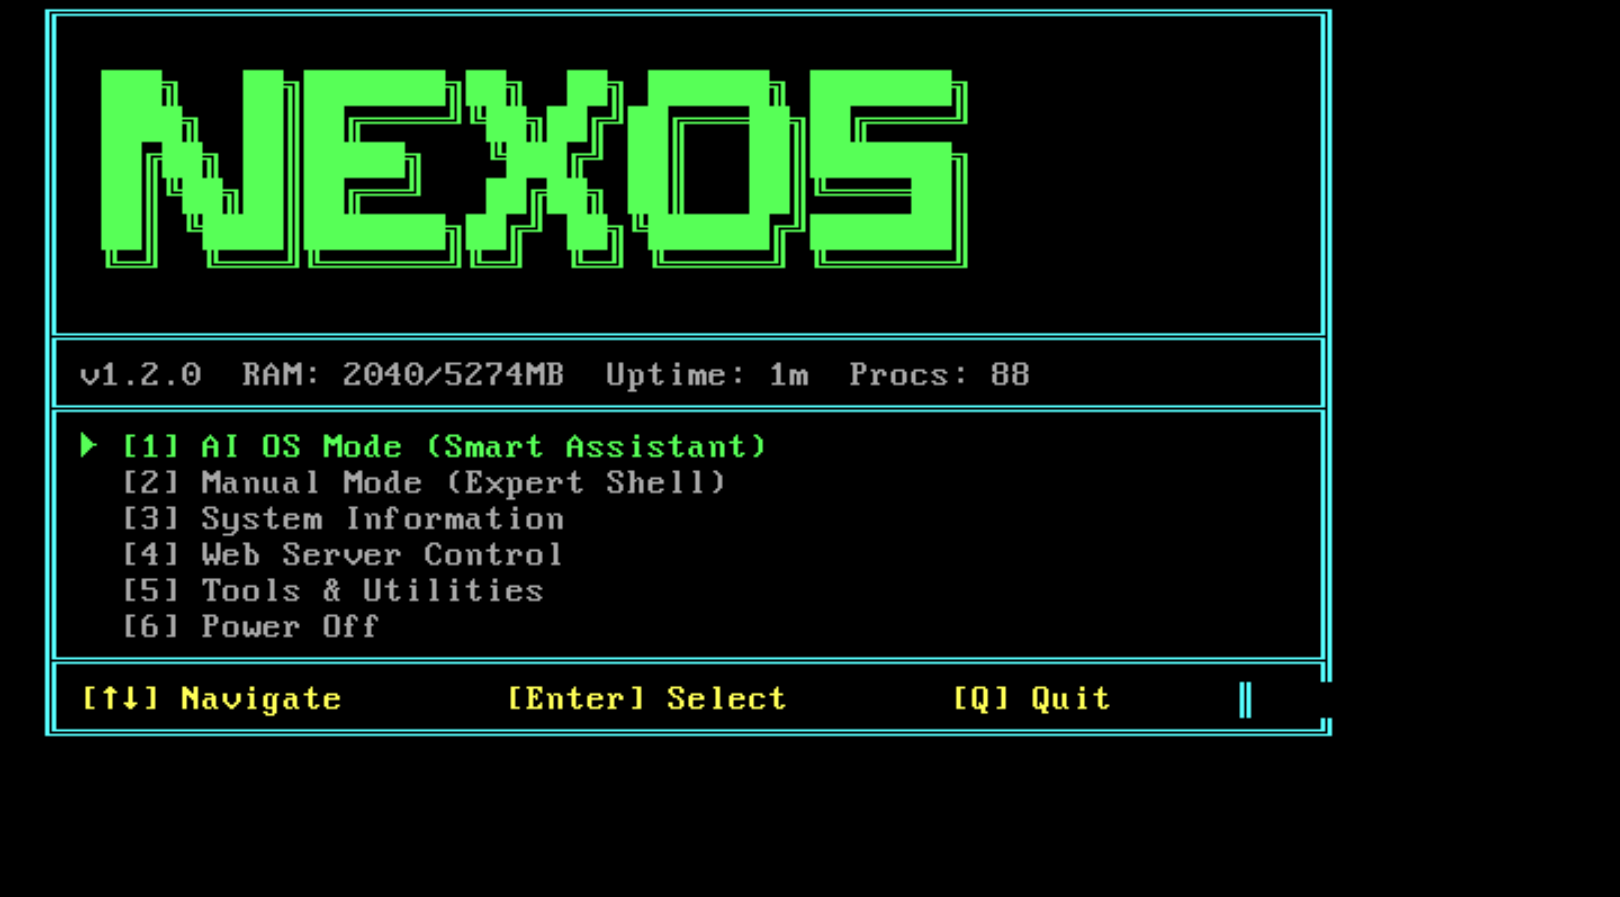
\includegraphics[width=0.8\textwidth]{images/dashboard.PNG}
\end{center}

\subsection{Yardım Sayfası}
\begin{center}
    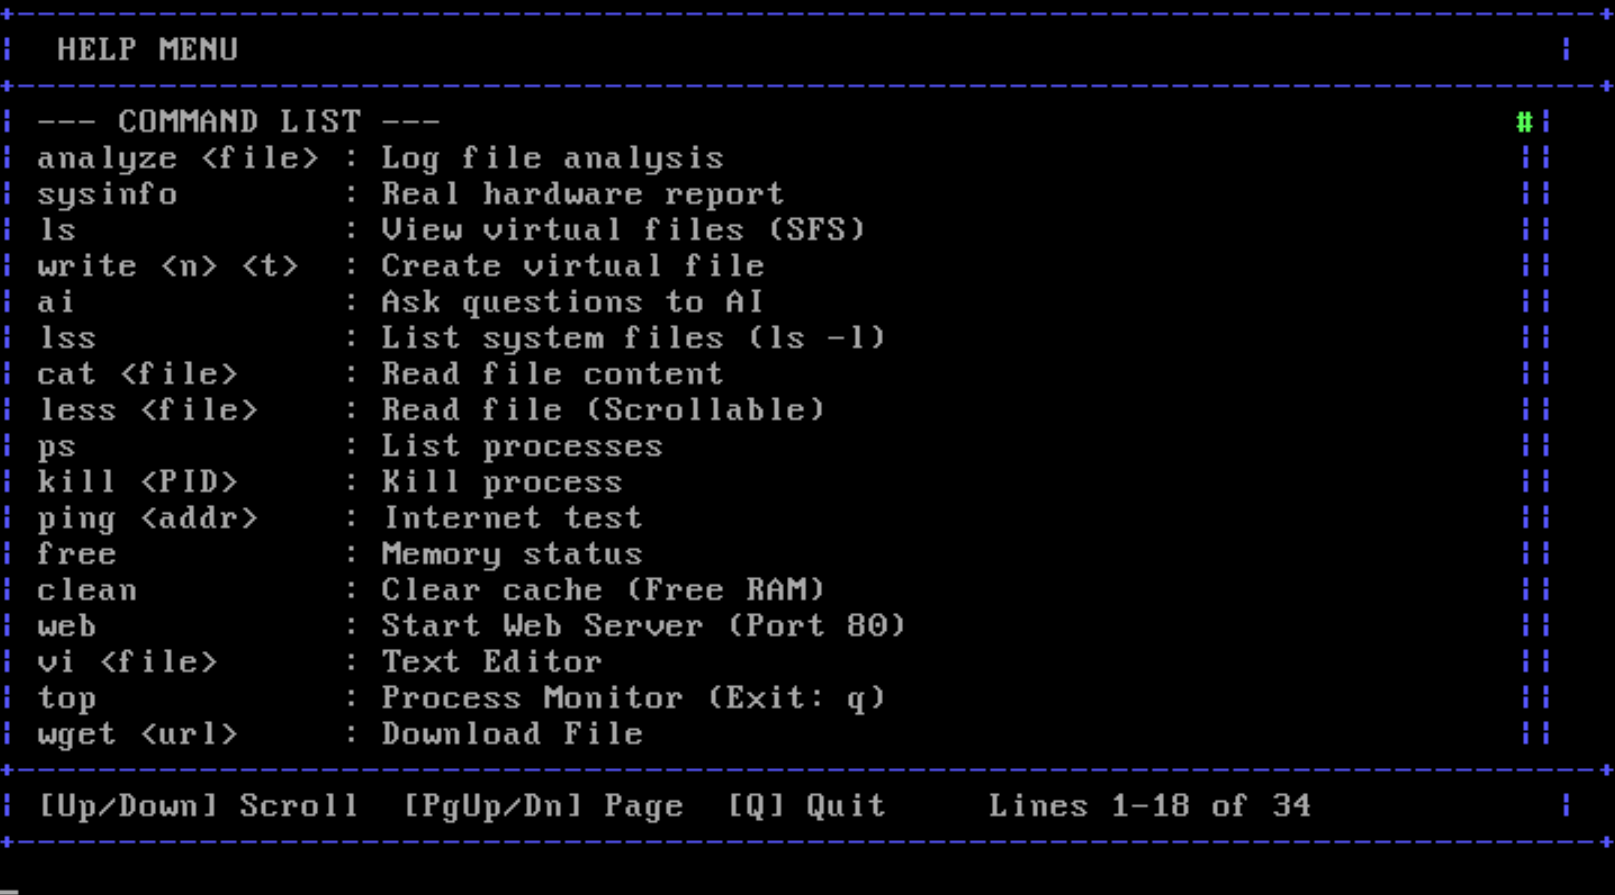
\includegraphics[width=0.8\textwidth]{images/help.PNG}
\end{center}

\subsection{Süreç Yönetimi (proc kill)}
\begin{center}
    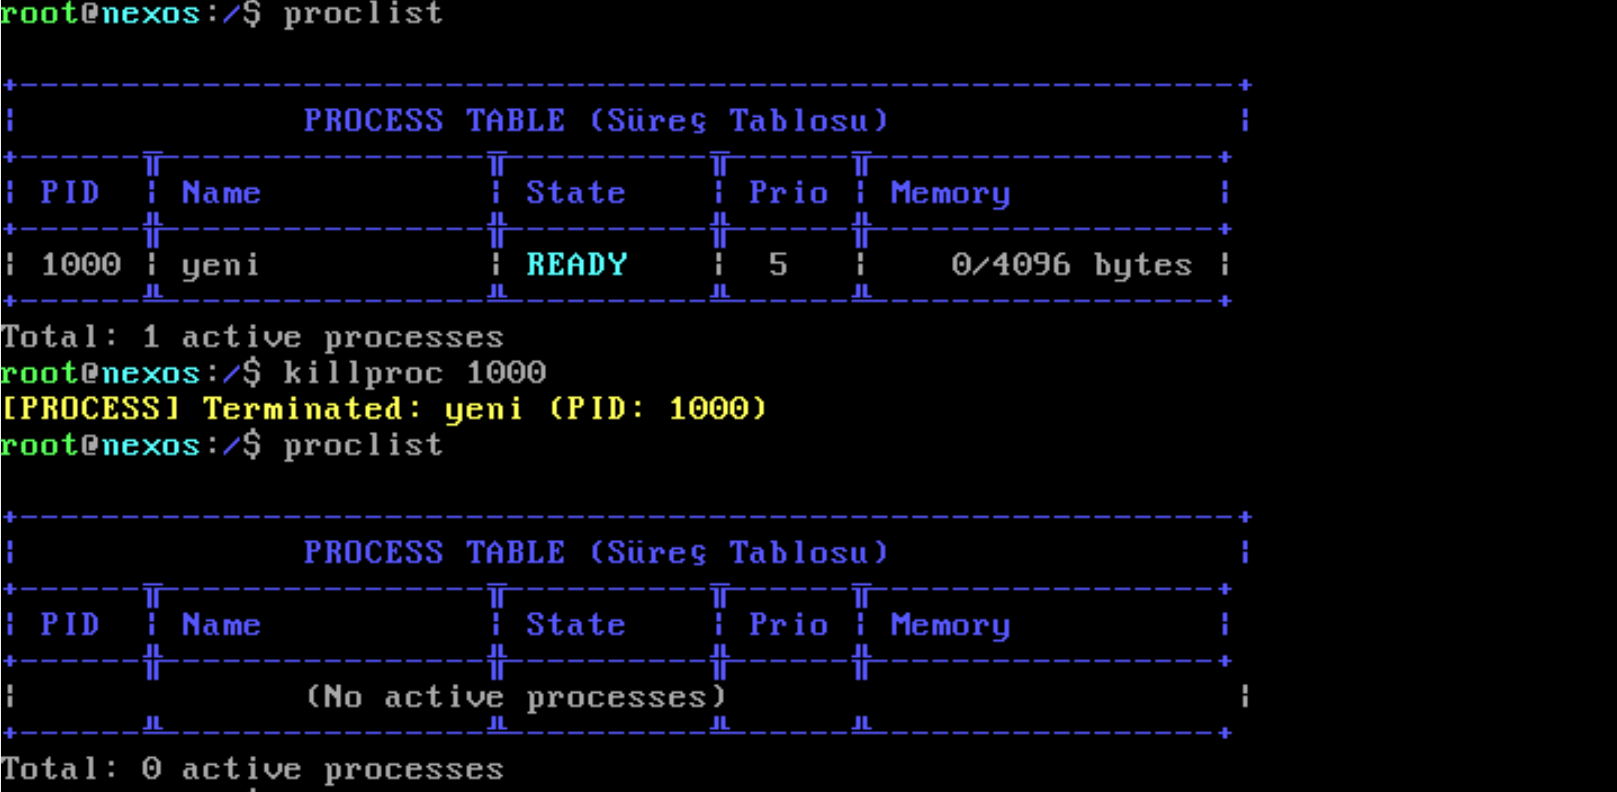
\includegraphics[width=0.8\textwidth]{images/proc_kill.PNG}
\end{center}

\subsection{Sistem İzleme (monitor)}
\begin{center}
    
\includegraphics[width=0.8\textwidth]{images/monitor.PNG}
\end{center}

\subsection{Log Analiz Çıktısı}
\begin{center}
    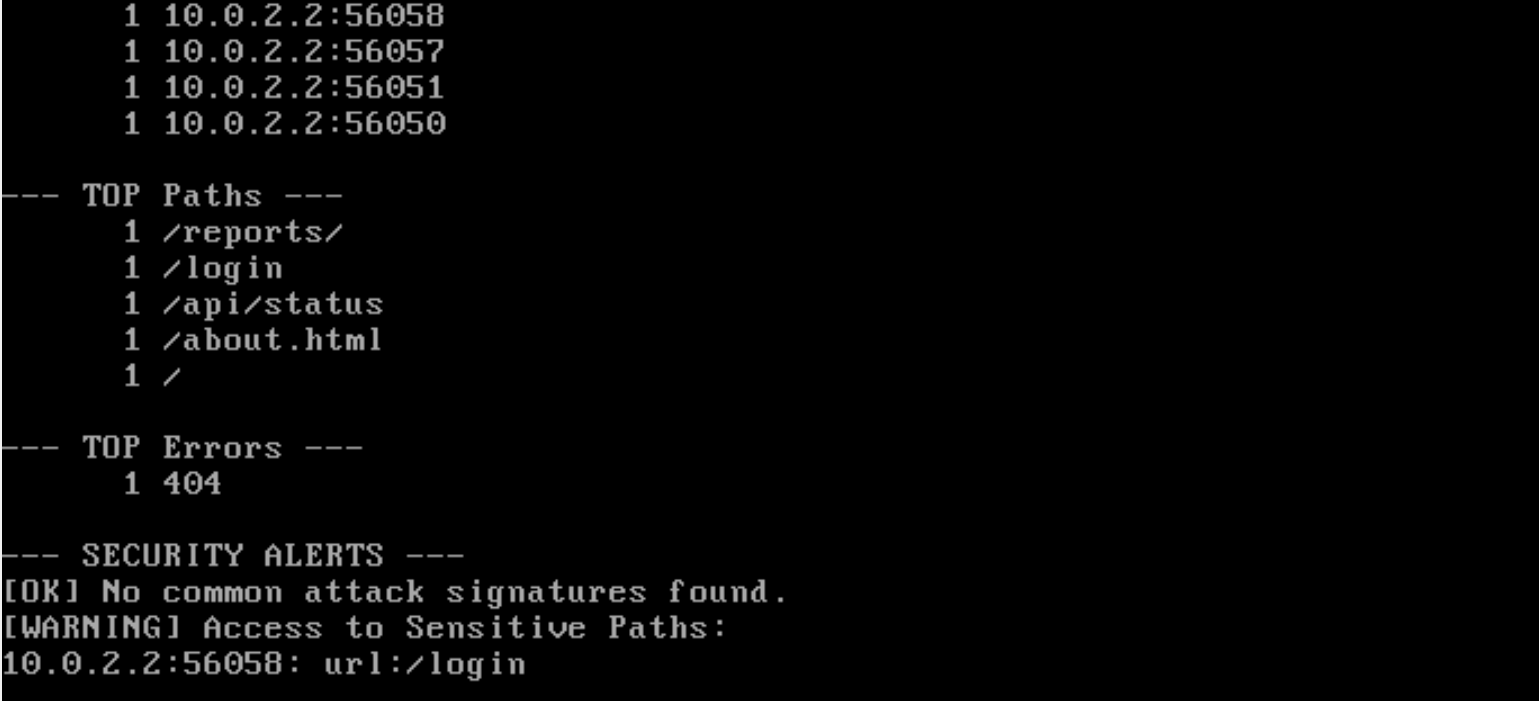
\includegraphics[width=0.8\textwidth]{images/analyze.PNG}
\end{center}



\subsection{Web Sitesi Görünümü}
\begin{center}
    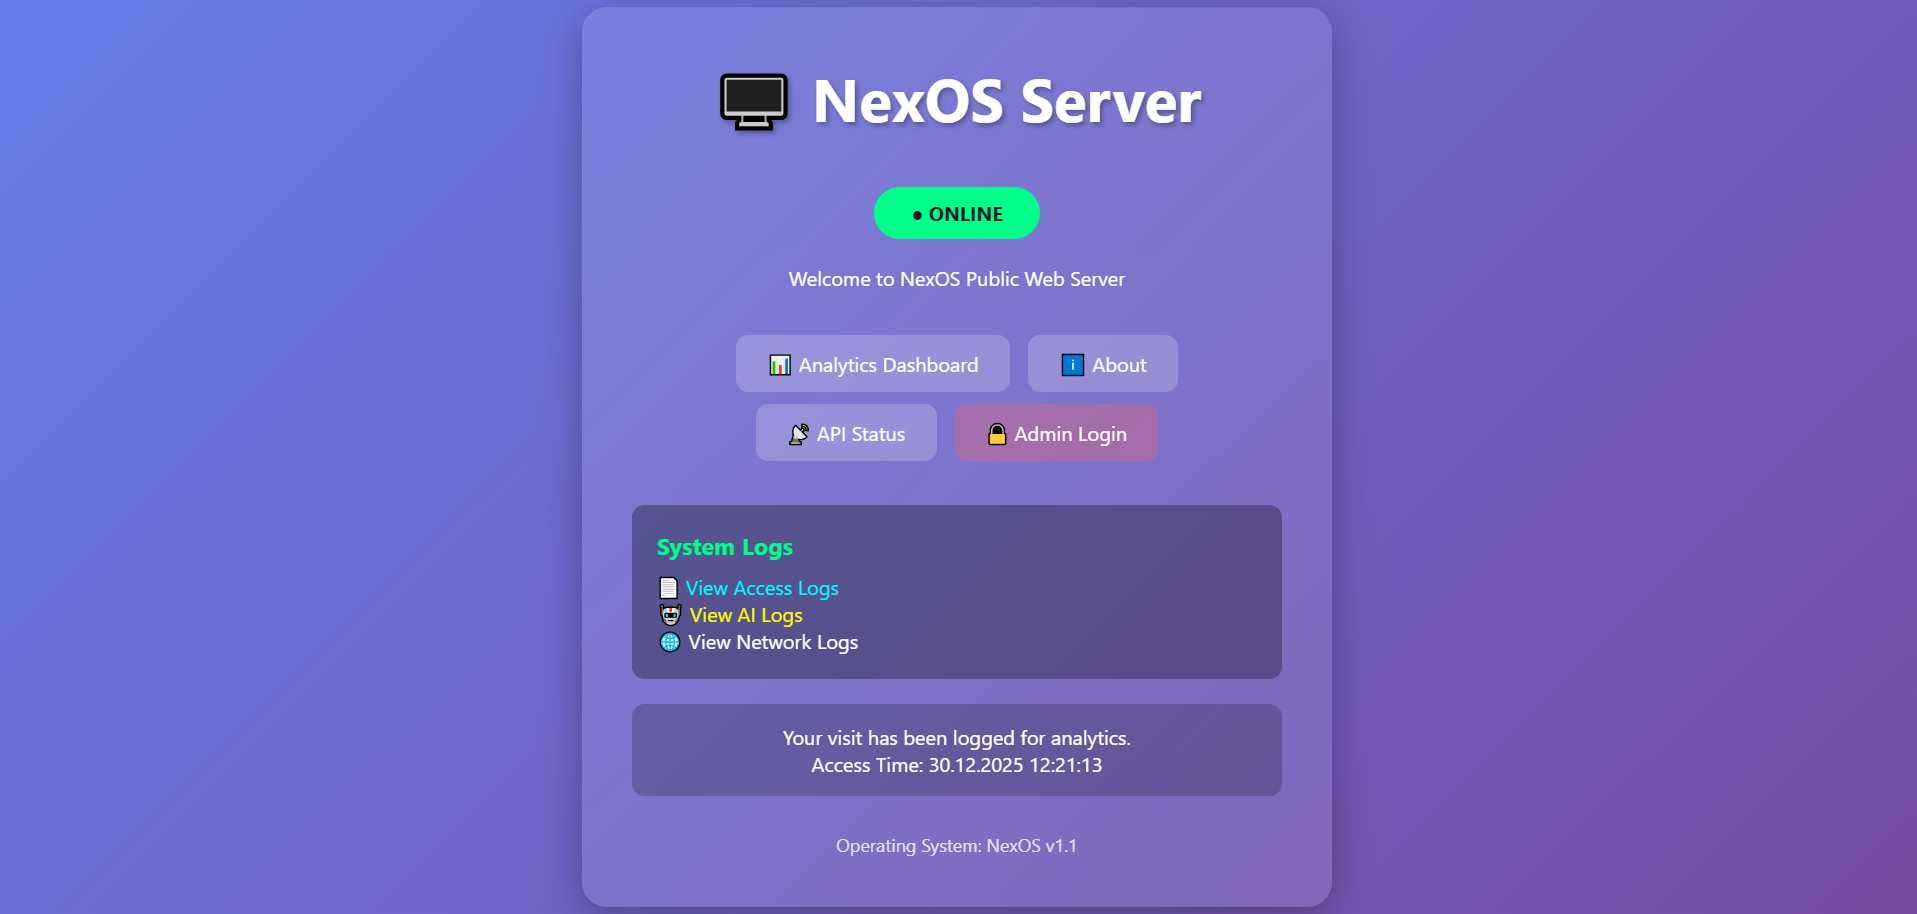
\includegraphics[width=0.9\textwidth]{images/serverweb.PNG}
\end{center}

\subsection{Yapay Zeka Yanıtı}
\begin{center}
    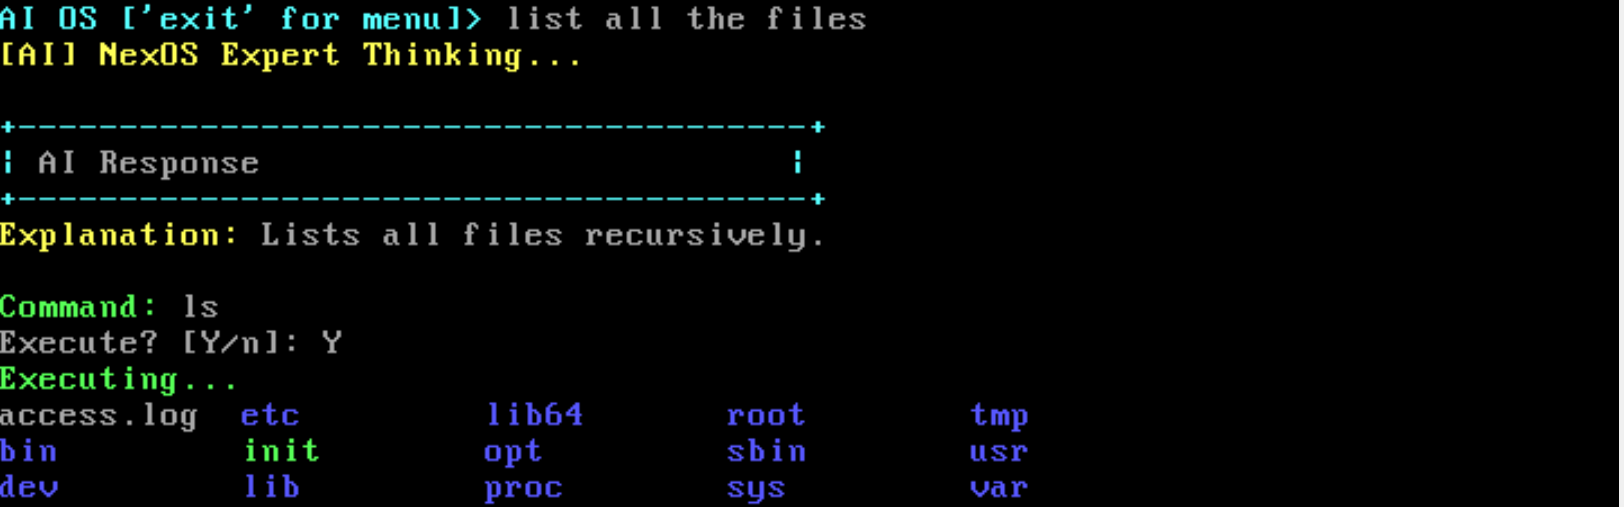
\includegraphics[width=0.9\textwidth]{images/airesponse.PNG}
\end{center}

\end{document}
